\documentclass[a4paper]{article}

\usepackage[pdftex,
  hidelinks,
  pdfauthor={Dexter Chua},
  pdfsubject={Cambridge Maths Notes: Part IA - Numbers and Sets},
  pdftitle={Part IA - Numbers and Sets},
pdfkeywords={Cambridge Mathematics Maths Math IA Michaelmas Numbers and Sets}]{hyperref}

\title{Part IA - Numbers and Sets}
\author{Lectured by A. G. Thomason\\\small Notes taken by Dexter Chua}
\date{Michaelmas 2014}

% Imports
\ifx \nextra \undefined
  \usepackage[pdftex,
    hidelinks,
    pdfauthor={Dexter Chua},
    pdfsubject={Cambridge Maths Notes: Part \npart\ - \ncourse},
    pdftitle={Part \npart\ - \ncourse},
  pdfkeywords={Cambridge Mathematics Maths Math \npart\ \nterm\ \nyear\ \ncourse}]{hyperref}
  \title{Part \npart\ - \ncourse}
\else
  \usepackage[pdftex,
    hidelinks,
    pdfauthor={Dexter Chua},
    pdfsubject={Cambridge Maths Notes: Part \npart\ - \ncourse\ (\nextra)},
    pdftitle={Part \npart\ - \ncourse\ (\nextra)},
  pdfkeywords={Cambridge Mathematics Maths Math \npart\ \nterm\ \nyear\ \ncourse\ \nextra}]{hyperref}

  \title{Part \npart\ - \ncourse \\ {\Large \nextra}}
\fi

\author{Lectured by \nlecturer \\\small Notes taken by Dexter Chua}
\date{\nterm\ \nyear}

\usepackage{alltt}
\usepackage{amsfonts}
\usepackage{amsmath}
\usepackage{amssymb}
\usepackage{amsthm}
\usepackage{booktabs}
\usepackage{caption}
\usepackage{enumitem}
\usepackage{fancyhdr}
\usepackage{graphicx}
\usepackage{mathtools}
\usepackage{microtype}
\usepackage{multirow}
\usepackage{pdflscape}
\usepackage{pgfplots}
\usepackage{siunitx}
\usepackage{tabularx}
\usepackage{tikz}
\usepackage{tkz-euclide}
\usepackage[normalem]{ulem}
\usepackage[all]{xy}

\pgfplotsset{compat=1.12}

\pagestyle{fancyplain}
\lhead{\emph{\nouppercase{\leftmark}}}
\ifx \nextra \undefined
  \rhead{
    \ifnum\thepage=1
    \else
      \npart\ \ncourse
    \fi}
\else
  \rhead{
    \ifnum\thepage=1
    \else
      \npart\ \ncourse\ (\nextra)
    \fi}
\fi
\usetikzlibrary{arrows}
\usetikzlibrary{decorations.markings}
\usetikzlibrary{decorations.pathmorphing}
\usetikzlibrary{positioning}
\usetikzlibrary{fadings}
\usetikzlibrary{intersections}
\usetikzlibrary{cd}

\newcommand*{\Cdot}{\raisebox{-0.25ex}{\scalebox{1.5}{$\cdot$}}}
\newcommand {\pd}[2][ ]{
  \ifx #1 { }
    \frac{\partial}{\partial #2}
  \else
    \frac{\partial^{#1}}{\partial #2^{#1}}
  \fi
}

% Theorems
\theoremstyle{definition}
\newtheorem*{aim}{Aim}
\newtheorem*{axiom}{Axiom}
\newtheorem*{claim}{Claim}
\newtheorem*{cor}{Corollary}
\newtheorem*{defi}{Definition}
\newtheorem*{eg}{Example}
\newtheorem*{fact}{Fact}
\newtheorem*{law}{Law}
\newtheorem*{lemma}{Lemma}
\newtheorem*{notation}{Notation}
\newtheorem*{prop}{Proposition}
\newtheorem*{thm}{Theorem}

\renewcommand{\labelitemi}{--}
\renewcommand{\labelitemii}{$\circ$}
\renewcommand{\labelenumi}{(\roman{*})}

\let\stdsection\section
\renewcommand\section{\newpage\stdsection}

% Strike through
\def\st{\bgroup \ULdepth=-.55ex \ULset}

% Maths symbols
\newcommand{\bra}{\langle}
\newcommand{\ket}{\rangle}

\newcommand{\N}{\mathbb{N}}
\newcommand{\Z}{\mathbb{Z}}
\newcommand{\Q}{\mathbb{Q}}
\renewcommand{\H}{\mathbb{H}}
\newcommand{\R}{\mathbb{R}}
\newcommand{\C}{\mathbb{C}}
\newcommand{\Prob}{\mathbb{P}}
\renewcommand{\P}{\mathbb{P}}
\newcommand{\E}{\mathbb{E}}
\newcommand{\F}{\mathbb{F}}
\newcommand{\cU}{\mathcal{U}}
\newcommand{\RP}{\mathbb{RP}}
\newcommand{\CP}{\mathbb{CP}}

\newcommand{\ph}{\,\cdot\,}

\DeclareMathOperator{\sech}{sech}
\DeclareMathOperator{\cosech}{cosech}
\DeclareMathOperator{\cosec}{cosec}

\DeclareMathOperator{\covol}{covol}
\DeclareMathOperator{\vol}{vol}

\let\Im\relax
\let\Re\relax
\DeclareMathOperator{\Im}{Im}
\DeclareMathOperator{\Re}{Re}
\DeclareMathOperator{\im}{im}
\DeclareMathOperator{\image}{image}
\DeclareMathOperator{\Ann}{Ann}

\DeclareMathOperator*{\res}{res}
\DeclareMathOperator{\Res}{Res}
\DeclareMathOperator{\Ind}{Ind}

\DeclareMathOperator{\tr}{tr}
\DeclareMathOperator{\diag}{diag}
\DeclareMathOperator{\rank}{rank}
\DeclareMathOperator{\card}{card}
\DeclareMathOperator{\spn}{span}
\DeclareMathOperator{\adj}{adj}

\DeclareMathOperator{\erf}{erf}
\DeclareMathOperator{\erfc}{erfc}

\DeclareMathOperator{\ord}{ord}
\DeclareMathOperator{\Sym}{Sym}

\DeclareMathOperator{\sgn}{sgn}
\DeclareMathOperator{\orb}{orb}
\DeclareMathOperator{\stab}{stab}
\DeclareMathOperator{\ccl}{ccl}

\DeclareMathOperator{\lcm}{lcm}
\DeclareMathOperator{\hcf}{hcf}

\DeclareMathOperator{\Int}{Int}
\DeclareMathOperator{\id}{id}

\DeclareMathOperator{\betaD}{beta}
\DeclareMathOperator{\gammaD}{gamma}
\DeclareMathOperator{\Poisson}{Poisson}
\DeclareMathOperator{\binomial}{binomial}
\DeclareMathOperator{\multinomial}{multinomial}
\DeclareMathOperator{\Bernoulli}{Bernoulli}
\DeclareMathOperator{\like}{like}

\DeclareMathOperator{\var}{var}
\DeclareMathOperator{\cov}{cov}
\DeclareMathOperator{\bias}{bias}
\DeclareMathOperator{\mse}{mse}
\DeclareMathOperator{\corr}{corr}

\DeclareMathOperator{\otp}{otp}
\DeclareMathOperator{\dom}{dom}

\DeclareMathOperator{\Root}{Root}
\DeclareMathOperator{\supp}{supp}
\DeclareMathOperator{\rel}{rel}
\DeclareMathOperator{\Hom}{Hom}
\DeclareMathOperator{\Aut}{Aut}
\DeclareMathOperator{\Gal}{Gal}
\DeclareMathOperator{\Mat}{Mat}
\DeclareMathOperator{\End}{End}
\DeclareMathOperator{\Char}{char}
\DeclareMathOperator{\ev}{ev}
\DeclareMathOperator{\St}{St}
\DeclareMathOperator{\Lk}{Lk}
\DeclareMathOperator{\disc}{disc}
\DeclareMathOperator{\Isom}{Isom}
\DeclareMathOperator{\length}{length}
\DeclareMathOperator{\energy}{energy}
\DeclareMathOperator{\area}{area}
\DeclareMathOperator{\Syl}{Syl}
\DeclareMathOperator{\cl}{cl}
\DeclareMathOperator{\fix}{fix}

\newcommand{\GL}{\mathrm{GL}}
\newcommand{\SL}{\mathrm{SL}}
\newcommand{\PGL}{\mathrm{PGL}}
\newcommand{\PSL}{\mathrm{PSL}}
\newcommand{\PSU}{\mathrm{PSU}}
\newcommand{\Or}{\mathrm{O}}
\newcommand{\SO}{\mathrm{SO}}
\newcommand{\U}{\mathrm{U}}
\newcommand{\SU}{\mathrm{SU}}

\renewcommand{\d}{\mathrm{d}}
\newcommand{\D}{\mathrm{D}}

\tikzset{->/.style = {decoration={markings,
                                  mark=at position 1 with {\arrow[scale=2]{latex'}}},
                      postaction={decorate}}}
\tikzset{<-/.style = {decoration={markings,
                                  mark=at position 0 with {\arrowreversed[scale=2]{latex'}}},
                      postaction={decorate}}}
\tikzset{<->/.style = {decoration={markings,
                                   mark=at position 0 with {\arrowreversed[scale=2]{latex'}},
                                   mark=at position 1 with {\arrow[scale=2]{latex'}}},
                       postaction={decorate}}}
\tikzset{->-/.style = {decoration={markings,
                                   mark=at position #1 with {\arrow[scale=2]{latex'}}},
                       postaction={decorate}}}
\tikzset{-<-/.style = {decoration={markings,
                                   mark=at position #1 with {\arrowreversed[scale=2]{latex'}}},
                       postaction={decorate}}}

\tikzset{circ/.style = {fill, circle, inner sep = 0, minimum size = 3}}
\tikzset{mstate/.style={circle, draw, blue, text=black, minimum width=0.7cm}}

\definecolor{mblue}{rgb}{0.2, 0.3, 0.8}
\definecolor{morange}{rgb}{1, 0.5, 0}
\definecolor{mgreen}{rgb}{0.1, 0.4, 0.2}
\definecolor{mred}{rgb}{0.5, 0, 0}

\def\drawcirculararc(#1,#2)(#3,#4)(#5,#6){%
    \pgfmathsetmacro\cA{(#1*#1+#2*#2-#3*#3-#4*#4)/2}%
    \pgfmathsetmacro\cB{(#1*#1+#2*#2-#5*#5-#6*#6)/2}%
    \pgfmathsetmacro\cy{(\cB*(#1-#3)-\cA*(#1-#5))/%
                        ((#2-#6)*(#1-#3)-(#2-#4)*(#1-#5))}%
    \pgfmathsetmacro\cx{(\cA-\cy*(#2-#4))/(#1-#3)}%
    \pgfmathsetmacro\cr{sqrt((#1-\cx)*(#1-\cx)+(#2-\cy)*(#2-\cy))}%
    \pgfmathsetmacro\cA{atan2(#2-\cy,#1-\cx)}%
    \pgfmathsetmacro\cB{atan2(#6-\cy,#5-\cx)}%
    \pgfmathparse{\cB<\cA}%
    \ifnum\pgfmathresult=1
        \pgfmathsetmacro\cB{\cB+360}%
    \fi
    \draw (#1,#2) arc (\cA:\cB:\cr);%
}
\newcommand\getCoord[3]{\newdimen{#1}\newdimen{#2}\pgfextractx{#1}{\pgfpointanchor{#3}{center}}\pgfextracty{#2}{\pgfpointanchor{#3}{center}}}

\def\Xint#1{\mathchoice
   {\XXint\displaystyle\textstyle{#1}}%
   {\XXint\textstyle\scriptstyle{#1}}%
   {\XXint\scriptstyle\scriptscriptstyle{#1}}%
   {\XXint\scriptscriptstyle\scriptscriptstyle{#1}}%
   \!\int}
\def\XXint#1#2#3{{\setbox0=\hbox{$#1{#2#3}{\int}$}
     \vcenter{\hbox{$#2#3$}}\kern-.5\wd0}}
\def\ddashint{\Xint=}
\def\dashint{\Xint-}


\begin{document}
\maketitle
{
  \small
  \noindent\textbf{Introduction to number systems and logic}\\
  Overview of the natural numbers, integers, real numbers, rational and irrational numbers, algebraic and transcendental numbers. Brief discussion of complex numbers; statement of the Fundamental Theorem of Algebra.

  \vspace{5pt}
  \noindent Ideas of axiomatic systems and proof within mathematics; the need for proof; the role of counter-examples in mathematics. Elementary logic; implication and negation; examples of negation of compound statements. Proof by contradiction.\hspace*{\fill}[2]

  \vspace{10pt}
  \noindent\textbf{Sets, relations and functions}\\
  Union, intersection and equality of sets. Indicator (characteristic) functions; their use in establishing set identities. Functions; injections, surjections and bijections. Relations, and equivalence relations. Counting the combinations or permutations of a set. The Inclusion-Exclusion Principle.\hspace*{\fill}[4]

  \vspace{10pt}
  \noindent\textbf{The integers}\\
  The natural numbers: mathematical induction and the well-ordering principle. Examples, including the Binomial Theorem.\hspace*{\fill}[2]

  \vspace{10pt}
  \noindent\textbf{Elementary number theory}\\
  Prime numbers: existence and uniqueness of prime factorisation into primes; highest common factors and least common multiples. Euclid’s proof of the infinity of primes. Euclid’s algorithm. Solution in integers of $ax+by = c$.

  \vspace{5pt}
  \noindent Modular arithmetic (congruences). Units modulo $n$. Chinese Remainder Theorem. Wilson's Theorem; the Fermat-Euler Theorem. Public key cryptography and the RSA algorithm.\hspace*{\fill}[8]

  \vspace{10pt}
  \noindent\textbf{The real numbers}\\
  Least upper bounds; simple examples. Least upper bound axiom. Sequences and series; convergence of bounded monotonic sequences. Irrationality of $\sqrt{2}$ and $e$. Decimal expansions. Construction of a transcendental number.\hspace*{\fill} [4]

  \vspace{10pt}
  \noindent\textbf{Countability and uncountability}\\
  Definitions of finite, infinite, countable and uncountable sets. A countable union of countable sets is countable. Uncountability of R. Non-existence of a bijection from a set to its power set. Indirect proof of existence of transcendental numbers.\hspace*{\fill}[4]}

\tableofcontents
\newpage
\section{Sets, functions and relations}
\subsection{Sets}
\begin{defi}[Set]
  A \emph{set} is a collection of stuff, without regards to order. Elements in a set are only counted once. eg. If $a = 2, b = c = 1$, then $A = \{a, b, c\}$ has only two members.
\end{defi}

\begin{defi}[Equality of sets]
  $A$ is equal to $B$, written as $A = B$, if 
  \[
    \forall x(x\in A \Leftrightarrow x\in B),
  \]
  ie. two sets are equal if they have the same elements.
\end{defi}

\begin{defi}[Subsets]
  $A$ is a \emph{subset} of $B$, written as $A\subseteq B$ or $A\subset B$, if all elements in $A$ are in $B$. ie. 
  \[
    \forall x(x\in A\Rightarrow x\in B).
  \]
\end{defi}

\begin{thm}
  $(A=B)\Leftrightarrow (A\subseteq B \text{ and }B\subseteq A)$
\end{thm}

Suppose $X$ is a set and $P$ is the property of some elements in $x$, we can write a set $\{x\in X:P(x)\}$ for the subset of $x$ comprising of the elements for which $P(x)$ is true. eg. $\{n\in \N : n \text{ is prime}\}$ is the set of all primes.

\begin{defi}[Intersection, union, set difference, symmetric difference and power set]
  Given two sets $A$ and $B$, we define the following:
  \begin{itemize}
    \item Intersection: $A\cap B = \{x:x\in A \text{ and } x\in B\}$
    \item Union: $A\cup B = \{x:x\in A\text{ or }x\in B\}$
    \item Set difference: $A\setminus B = \{x\in A: x\not\in B\}$
    \item Symmetric difference: $A\Delta B = \{x: x\in A\text{ xor } x\in B\}$, ie. the elements in exactly one of the two sets
    \item Power set: $\mathcal{P}(X) = \{X: X\subseteq P\}$, ie. the set of all subsets
  \end{itemize}
\end{defi}

\note New sets can only be created via the above operations on old sets (plus replacement, which says that you can replace an element of a set with another element). One cannot arbitrarily create sets such as $X=\{x:x\text{ is a set and }x\not\in x\}$. Otherwise paradoxes will arise.

\begin{prop}\leavevmode
  \begin{itemize}
    \item $(A\cap B)\cap C = A \cap (B\cap C)$
    \item $(A\cup B)\cup C = A\cup (B\cup C)$
    \item $A\cap(B\cup C) = (A\cap B)\cup (A\cap C)$
  \end{itemize}
\end{prop}

\begin{notation}
  If $A_\alpha$ are sets for all $\alpha \in I$, then 
  \[
    \bigcap_{\alpha\in I}A_\alpha = \{x:\forall\alpha\in I: x\in A_\alpha\}
  \]
  and
  \[
    \bigcup_{\alpha\in I}A_\alpha = \{x:\exists\alpha\in I: x\in A_\alpha\}.
  \]
\end{notation}

\begin{defi}[Ordered pair]
  An \emph{ordered pair} $(a, b)$ is a pair of two items in which order matters. Formally, it is defined as $\{\{a\}, \{a, b\}\}$. We have $(a, b) = (a', b')$ iff $a = a'$ and $b = b'$.
\end{defi}

\begin{defi}[Cartesian product]
  Given two sets $A, B$, the \emph{Cartesian product} of $A$ and $B$ is $A\times B = \{(a, b):a\in A, b\in B\}$. This can be extended to $n$ products, eg. $\R^3 = \R\times\R\times\R = \{(x,y,z): x, y, z\in \R\}$ (which is officially $\{(x, (y, z)): x, y, z\in \R\}$).
\end{defi}

\subsection{Functions}
\begin{defi}[Function/map]
  A \emph{function} (or \emph{map}) $f: A\to B$ is a ``rule'' that assigns, for each $a\in A$, precisely one element $f(a)\in B$. We can write $a\mapsto f(a)$. Formally, we say $f\subseteq A\times B$ such that $\forall a\in A$, there exists a unique $b\in B$ such that $(a, b)\in f$.
\end{defi}

\begin{eg}
  $\frac{1}{x}:\R\to\R$ is not a function since $f(0)$ is not defined. $\pm x: \R\to\R$ is also not a function since it is multi-valued.
\end{eg}

\begin{defi}[Injective function]
  A function $f$ is \emph{injective} if it hits everything at most once, ie.
  \[
    \forall x, y\in X(f(x) = f(y)\Rightarrow x = y)
  \]
\end{defi}

\begin{defi}[Surjective function]
  A function is \emph{surjective} if it hits everything at least once, ie. 
  \[
    \forall y\in Y(\exists x\in X(f(x) = y))
  \]
\end{defi}

\begin{eg}
  $f: \R \to\R^+\cup\{0\}$ with $x \mapsto x^2$ is surjective but not injective.
\end{eg}

\begin{defi}[Bijective function]
  A function is \emph{bijective} if it is both injective and surjective. ie. it hits everything exactly once. Note that a function has an inverse iff it is bijective.
\end{defi}

\begin{defi}[Permutation (function)]
  A \emph{permutation} of $A$ is a bijection $A\to A$.
\end{defi}

\begin{defi}[Composition of functions]
  The \emph{composition} of two functions is a function you get by applying one after another. In particular, if $f: X \rightarrow Y$ and $G: Y\rightarrow Z$, then $g\circ f: X \rightarrow Z$ with $g\circ f(x) = g(f(x))$. Note that function composition is associative.
\end{defi}

\begin{defi}[Image of function]
  If $f: A\to B$ and $U\subseteq A$, then $f(U) = \{f(u):u\in U\}$.

  $f(A)$ is the \emph{image} of $A$. We have $f$ is surjective iff $f(A) = B$.
\end{defi}

\begin{defi}[Pre-image of function]
  If $f: A\to B$ and $V\subseteq B$, then $f^{-1}(V) = \{a\in A: f(a)\in V\}$.
\end{defi}

\begin{defi}[Identity map]
  The \emph{identity map} $\id _A: A\to A$ is defined as the map $a\mapsto a$.
\end{defi}

\begin{defi}[Left inverse of function]
  Given $f: A\to B$, a \emph{left inverse} of $f$ is a function $g:B\to A$ such that $g\circ f = \id _A$.
\end{defi}

\begin{defi}[Right inverse of function]
  Given $f: A\to B$, a \emph{right inverse} of $f$ is a function $g:B\to A$ such that $f\circ g = \id _B$.
\end{defi}

\begin{thm}
  The left inverse of $A$ exists iff $f$ is injective.
\end{thm}

\begin{proof}
  ($\Rightarrow$)
  If the left inverse $g$ exists, then $\forall a, a'\in A, f(a) = f(a') \Rightarrow g(  f(a))=g(f(a'))\Rightarrow a=a'$. Therefore $f$ is injective.

  ($\Leftarrow$) if $f$ is injective, we can construct a $g$ defined as
  \[
    g: \begin{cases}
      g(b) = a &\text{if }b\in f(A), \text{ where }f(a) = b\\
      g(b) = \text{anything} & \text{otherwise}
    \end{cases}.
  \]
  Then $g$ is a left inverse of $f$.
\end{proof}

\begin{thm}
  The right inverse of $A$ exists iff $f$ is surjective.
\end{thm}

\begin{proof}
  ($\Rightarrow$) We have $f(g(B)) = B$ since $f\circ g$ is the identity function. Thus $f$ must be surjective since its image is $B$.

  ($\Leftarrow$) If $f$ is surjective, we can construct a $g$ such that for each $b\in B$, pick one $a\in A$ with $f(a) = b$, and put $g(b) = a$.

  \note This proof relies on the Axiom of Choice. In fact, this ``theorem'' is equivalent to the axiom of choice.

  Assume any surjective function $f$ has a right inverse. Given a family of non-empty sets $A_i$ for $i\in I$ (wlog assume they are disjoint), define a function $f: \bigcup A_i \to I$ that sends each element to the set that contains the element. This is surjective since each set is non-empty. Then it has a right inverse. Then the right inverse must send each set to an element in the set, ie. is a choice function for $A_i$.
\end{proof}

\begin{defi}[Inverse of function]
  An \emph{inverse} of $f$ is a function that is both a left inverse and a right inverse. It is written as $f^{-1}: B\to A$. It exists if $f$ is bijective, and is necessarily unique.
\end{defi}

\subsection{Relations}
\begin{defi}[Relation]
  A \emph{relation} $R$ on $A$ specifies that some elements of $A$ are related to some others. Formally, $R\subseteq A\times A$. We write $aRb$ iff $(a, b)\in R$.
\end{defi}

\begin{eg}
  The following are examples of relations on natural numbers:
  \begin{enumerate}
    \item $aRb$ iff $a$ and $b$ have the same final digit. eg. $(37)R(57)$.
    \item $aRb$ iff $a$ divides $b$. eg. $2R6$ and $2\not \!\!R 7$.
    \item $aRb$ iff $a\not= b$.
    \item $aRb$ iff $a = b = 1$.
    \item $aRb$ iff $|a - b|\leq 3$.
    \item $aRb$ iff either $a, b\geq 5$ or $a, b\leq 4$.
  \end{enumerate}
\end{eg}

\begin{defi}[Reflexive relation]
  A relation $R$ is \emph{reflexive} if $\forall a(aRa)$.
\end{defi}

\begin{defi}[Symmetric relation]
  A relation $R$ is \emph{symmetric} iff $\forall a, b(aRb\Leftrightarrow bRa)$.
\end{defi}

\begin{defi}[Transitive relation]
  A relation $R$ is \emph{transitive} iff $\forall a, b, c(aRb\vee bRc \Rightarrow aRc)$.
\end{defi}

\begin{eg}
  With regards to the examples above,

  \vspace{4pt}
  \noindent
  \begin{tabular}{lcccccc}
    \toprule
    Examples   & (i)        & (ii)       & (iii)      & (iv)       & (v)        & (vi)       \\
    \midrule
    Reflexive  & \checkmark & \checkmark & $\times$   & $\times$   & \checkmark & \checkmark \\
    Symmetric  & \checkmark & $\times$   & \checkmark & \checkmark & \checkmark & \checkmark \\
    Transitive & \checkmark & \checkmark & $\times$   & \checkmark & $\times$   & \checkmark \\
    \bottomrule
  \end{tabular}
\end{eg}

\begin{defi}[Equivalence relation]
  A relation is an \emph{equivalence relation} if it is reflexive, symmetric and transitive. eg. (i) and (vi) in the above examples are equivalence relations.
\end{defi}
\note If it is an equivalence relation, we usually write $\sim$ instead of $R$.
\begin{eg}
  If we consider a deck of cards, define two cards to be related if they have the same suite.
\end{eg}

\begin{defi}[Partition of set]
  A \emph{partition} of a set $X$ is a collection of subsets $A_\alpha$ of $X$ such that each element of $X$ is in exactly one of $A_\alpha$.
\end{defi}

\begin{defi}[Equivalence class]
  If $\sim$ is an equivalence relation, then the \emph{equivalence class} $[x]$ is the set of all elements that are related via $\sim$ to $x$.
\end{defi}

\begin{eg}
  In the cards example, $[8\heartsuit] = \{\heartsuit\}$.
\end{eg}

\begin{thm}
  If $\sim$ is an equivalence relation on $A$, the equivalence classes of $\sim$ form a partition of $A$.
\end{thm}

\begin{proof}
  By reflexivity, we have $a\in [a]$. Thus the equivalence classes cover the whole set. We must now show that for all $a, b\in A$, either $[a] = [b]$ or $[a]\cap [b]=\emptyset$.

  Suppose $[a]\cap[b]\not=\emptyset$. Then $\exists c\in [a]\cap[b]$. So $a\sim c, b\sim c$. By symmetry, $c\sim b$. By transitivity, we have $a\sim b$. For all $b'\in [b]$, we have $b\sim b'$. Thus by transitivity, we have $a\sim b'$. Thus $[b]\subseteq[a]$. By symmetry, $[a]\subseteq[b]$  and $[a] = [b]$.
\end{proof}

On the other hand, each partition defines an equivalence relation in which two elements are related iff they are in the same partition. Thus partitions and equivalence relations are ``the same thing''.
\begin{defi}[Quotient map]
  The \emph{quotient map} $q$ maps each element in $A$ to the equivalence class containing $a$, ie. $a\mapsto [a]$. eg. $q(8\heartsuit) = \{\heartsuit\}$.
\end{defi}

\section{Division}
\subsection{Euclid's Algorithm}
\begin{defi}[Factor of integers]
  Given $a, b\in \Z$, we say $a$ \emph{divides} $b$, $a$ is a \emph{factor} of $b$ or $a|b$ if $\exists c\in \Z(b = ac)$. For any $b$, $\pm 1$ and $\pm b$ are always factors of $b$. The other factors are called \emph{proper factors}
\end{defi}

\begin{thm}[Division Algorithm]
  Given $a, b\in \Z$, there are unique $q, r\in \Z$ with $a = qb + r$ and $0\leq r < b$.
\end{thm}

\begin{proof}
  Choose $q = \max\{q:qb \leq n\}$. This maximum exists because the set of all $q$ such that $qb\leq n$ is finite. Now write $r = a - qb$. We have $0\leq r < b$ and thus $q$ and $r$ are found.

  To show that they are unique, suppose that $a = qb + r = q'b + r'$. We have $(q - q')b = (r' - r)$. Since both $r$ and $r'$ are between $0$ and $b$, we have $-b < r - r' < b$. However, $r' - r$ is a multiple of $b$. Thus $q - q' = r' - r = 0$. Consequently, $q = q'$ and $r = r'$.
\end{proof}

\begin{defi}[Common factor of integers]
  A \emph{common factor} of $a$ and $b$ is a number $c\in\Z$ such that $c|a$ and $c|b$.
\end{defi}

\begin{defi}[Highest common factor/greatest common divisor]
  The \emph{highest common factor} or \emph{greatest common divisor} of two numbers $a, b\in \N$ is a number $d\in \N$ such that $d$ is a common factor of $a$ and $b$, and if $c$ is also a common factor, $c|d$.

  Clearly if the hcf exists, it must be the largest common factor, since all other common factors divide it, and thus necessarily unique.
\end{defi}
\note You might think reasonably it is more natural to define $\hcf(a, b)$ to be the largest common factor. Then show that it has the property that all common factors divide it. But the above definition is superior because it does not require a prior ordering of the natural numbers, and can be extended to any ring even if they are not ordered.

\begin{notation}
  We write $d = \hcf(a, b) = \gcd(a, b) = (a, b)$.

  \note here we use $(a, b)$ to stand for a number, and has nothing to do with an ordered pair.
\end{notation}

\begin{prop}
  If $c|a$ and $c|b$, $c|(ua + vb)$ for all $u, v\in \Z$.
\end{prop}

\begin{proof}
  By definition, we have $a = kc$ and $b = lc$. Then $ua + vb = ukc + vlc = (uk + vl)c$ and $c|(ua + vb)$.
\end{proof}

\begin{thm}
  Let $a,b\in \N$. Then $(a, b)$ exists.
\end{thm}

\begin{proof}
  Let $S=\{ua + vb:i, v\in\Z\}$ be the set of all linear combinations of $a, b$. Let $d$ be the smallest positive member of $S$. Say $d = xa + yb$. If $c|a, c|b$, then $c|d$. So we need to show that $d|a$ and $d|b$, and thus $d=(a, b)$.

  By the division algorithm, there exists numbers $q, r\in\Z$ with $a = qd + r$ with $0\leq r < d$. Then $r = a - qd = a(1 - qx) - qyb$. Therefore $r$ is a linear combination of $a$ and $b$. Since $d$ is the smallest positive member of $S$ and $0\leq r < d$, we have $r = 0$ and $d|a$. Similarly, we can show that $d|b$.
\end{proof}

\begin{cor}
  (from the proof) Let $d  = (a, b)$, then $d$ is the smallest positive linear combination of $a$ and $b$.
\end{cor}

\begin{cor}[B\'{e}zout's identity]
  Let $a, b\in\N$ and $c\in Z$. Then there exists $u, v\in \Z$  with $c=ua + vb$ iff $(a, b)|c$.
\end{cor}

\begin{proof}
  ($\Rightarrow$) Let $d=(a, b)$. If $c$ is a linear combination of $a$ and $b$, then $d|c$ because $d|a$ and $d|b$.

  ($\Leftarrow$) Suppose that $d|c$. Let $d = xa + yb$ and $c = kd$. Then $c = (kx)a + (ky)b$. Thus $c$ is a linear combination of $a$ and $b$.
\end{proof}

Note that the proof above is existential, not constructive. How can we actually find $d$, and how can we find $x, y$ such that $d = xa + yb$?

While it might be easy to simply inspect $d$ for small numbers, how would you find common factors of, say, 4931 and 3795? We cannot use primes because (a) prime factorization is hard; and (b) primes are not yet defined.

You might spot if $c|4931$ and $c|3795$, then $c|(4931 - 3795)=1136$. The process is also reversible - if $c|1136$ and $c|3795$, then $c|(1136 + 3795) = 4931$). Thus the problem is equivalent to finding common factors of $3795$ and $1136$. The process can be repeated until we have small numbers.

\begin{prop}[Euclid's Algorithm]
  If we continuously break down $a$ and $b$ by the following procedure: 
  \begin{align*}
    a &= q_1b + r_1\\
    b &= q_2r_1 + r_2\\
    r_1 &= q_3r_2 + r_3\\
    &\vdots\\
    r_{n-2} &= q_nr_{n-1}
  \end{align*}
  then the highest common factor is $r_{n-1}$.
\end{prop}

\begin{proof}
  We have common factors of $a, b=$ common factors of $b, r_1=$ common factors of $r_1, r_2 = \cdots = $ factors of $r_{n-1}$.
\end{proof}
\note This gives an alternative proof that hcfs exist.

\note We have $a\geq b + r_1 > 2r_1$. Thus every two steps, the number on the left goes down by at least half. Hence the number of digits goes down every 8 steps. Thus the time needed is $\leq 8\times$ number of digits and has time complexity $O(\log b)$.

\begin{eg}
  Suppose $a = 57$ and $b = 42$. \\
  \begin{tabular}{l l l}
    common factors of $57$ and $42$   &  & $57 = 1\times 42 + 15$ \\
    = common factors of $42$ and $15$ &  & $42 = 2\times 15 + 12$ \\
    = common factors of $15$ and $12$ &  & $15 = 1\times 12 + 3$  \\
    = common factors of $12$ and $3$  &  & $12 = 4\times 3 + 0$   \\
    = common factors of $3$ and $0$                               \\
    = factors of $3$.
  \end{tabular}
\end{eg}

By reversing Euclid's Algorithm, we can find the hcf of two numbers as a linear combination of $a$ and $b$.
\begin{eg}
  Consider $57$ and $21$.
  \begin{align*}
    57 &= 2\times 21 + 15\\
    21 &= 1\times 15 + 6\\
    15 &= 2\times 6 + 3\\
    6 &= 2\times 3
  \end{align*}

  In the opposite direction, we have
  \begin{align*}
    3 &= 15 - 2\times 6\\
    &= 15 - 2\times (21 - 15)\\
    &= 3\times 15 - 2\times 21\\
    &= 3\times (57 - 2\times 21) - 2\times 21\\
    &= 3\times 57 - 5\times 21
  \end{align*}
\end{eg}

This gives an alternative constructive proof of B\'{e}zout's identity. Moreover, it gives us a quick way of expressing $(a, b) = ax + by$. However, this algorithm requires storing the whole process of Euclid's Algorithm and is not efficient space-wise.

For higher space efficiency, Write $A_{-1} = 0$, $A_0 = 1$. $B_{-1} = 1$, $B_0 = 0$. For $j \geq 1$, write
\begin{align*}
  A_j &= q_jA_{j-1} + A_{j - 2}\\
  B_j &= q_jB_{j-1} + B_{j-1}
\end{align*}
where $q_j$ is the $j$-th quotient in the Euclid's Algorithm. Then
\[
  a\times B_j - b\times A_j = (-1)^{j-1}r_j.
\]
In particular, $a\times B_{n-1} - b\times A_{b-1} = (-1)^{n-1}r_{n - 1} = (a, b)$.

Also, $A_jB_{j - 1} - B_jA_{j-1} = (-1)^j$. So $(A_j, B_j) = 1$.

Putting the Euclid's Algorithm's equations in the following form, 
\begin{align*}
  \frac{57}{21} &= 2 + \frac{15}{21}\\
  \frac{21}{15} &= 1 + \frac{6}{15}\\
  \frac{15}{6} &= 2 + \frac{3}{6}\\
  \frac{6}{3} &= 2
\end{align*}

We have 
\[
  \frac{57}{21} = 2 + \cfrac{1}{1 + \cfrac{1}{2 + \cfrac{1}{2}}}
\]
Expanding this continued fractions, we can have the sequence, $2, 2 + \frac{1}{1} = 3$, $2 + \frac{1}{1 + \frac{1}{2}} = \frac{8}{3}$ (These are called the ``convergents''). The series happens to be $\frac{A_i}{B_i}$.

\subsection{Primes}
\begin{defi}[Prime number]
  $p\in \N$ is a \emph{prime} if $p > 1$ and the only factors of $p$ are $\pm 1$ and $\pm p$.
\end{defi}

\begin{thm}
  Every number can be written as a product of primes.
\end{thm}

\begin{proof}
  If $n\in \N$ is not a prime itself, then by definition $n = ab$. If either $a$ or $b$ is not prime, then that number can be written as a product, say $b = cd$. Then $n = acd$ and so on. (Rigorous proof by strong induction) Since these numbers are getting smaller, and the process will stop when they are all prime.
\end{proof}

\begin{thm}
  There are infinitely many primes.
\end{thm}

\begin{proof}
  (Euclid's proof) Suppose there are finitely many primes, say $p_1, p_2 \cdots p_n$. Then $N = p_1p_2\cdots p_n + 1$ is divisible by none of the primes.  Otherwise, $p_j|(N - p_1p_2\cdots p_n)$, ie. $p_j|1$, which is impossible. However, $N$ is a product of prime, so there must be primes not amongst $p_1, p_2\cdots p_n$.
\end{proof}

\begin{proof}
  (Erd\"{o}s 1930) Suppose that there are finitely many primes, $p_1, p_2\cdots p_n$. Consider all numbers that are the products of these primes, ie. $p_1^{j_1}p_2^{j_2}\cdots p_n^{j_n}$, where $k_i \geq 0$. Factor out all squares to obtain the form $m^2p_1^{i_1}p_2^{i_2}\cdots p_n^{i_n}$, where $m\in \N$ and $i_k = 0$ or $1$.

  Let $N\in\N$. Given any number $x \leq N$, when put in the above form, we have $m \leq \sqrt{N}$. So there are at most $\sqrt{N}$ possible values of $m$. For each $m$, there are $2^k$ numbers of the form $m^2p_1^{i_1}p_2^{i_2}\cdots p_n^{i_n}$. So there are only $\sqrt{N}\times 2^k$ possible values of $x$ of this kind.

  Now pick $N\geq 4^k$. Then $N > \sqrt{N}\times 2^k$. So there must be a number $\leq N$ not of this form, ie. it has a prime factor not in this list.
\end{proof}

\note Euclid says \emph{this} number $N$ has \emph{all} prime factors not in the list. Erd\"{o}s says that \emph{some} number has \emph{some} prime factors not in the list. Also, Euclid's shows that the $k$-th prime $< 2^{2^k}$ (by induction), while Erd\"{o}s shows that the $k$-th prime $<4^k$. (In fact prime number theorem says that the $k$-th prime $\sim k\log k$).

\begin{thm}
  If $a| bc$ and $(a, b) = 1$, then $a | c$.
\end{thm}

\begin{proof}
  From Euclid's algorithm, there exists integers $u, v\in \Z$ such that $ua + vb = 1$. So multiplying by $c$,  we have $uac + vbc = c$. Now $a | $LHS. So $a | c$.
\end{proof}

\begin{defi}[Coprime numbers]
  We say $a, b$ are \emph{coprime} if $(a, b) = 1$. 
\end{defi}

\begin{cor}
  If $p$ is a prime and $p|ab$, then $p|a$ or $p|b$. (True for all $p, a, b$)
\end{cor}

\begin{proof}
  Consider $(p, a) = p$ or $1$ because $p$ is a prime. If $(p, a) = p$, then $p | a$. Otherwise, $(p, a) = 1$ and $p | b$ by the theorem above.
\end{proof}

\begin{cor}
  If $p$ is a prime and $p|n_1n_2\cdots n_i$, then $p | n_i$ for some $i$. 
\end{cor}

\note The \emph{definition} of prime is about stuff $ | p$. The above corollary is above $p | $\,stuff.

\begin{thm}[Fundamental Theorem of Arithmetic]
  Every natural number is expressible as a product of primes in exactly one way. In particular, if $p_1p_2\cdots p_k = q_1q_2\cdots q_l$, where $p_i, q_i$ are primes but not necessarily distinct, then $k = l$. $q_1, \cdots q_l$ are $p_1, \cdots p_k$ in some order. Since we already showed at least one way above, we only need to show uniqueness.
\end{thm}

\begin{proof}
  Let $p_1\cdots p_k = q_1\cdots q_l$. We know that $p_1 | q_1\cdots q_l$. Then $p_1 | q_1(q_2q_3\cdots q_l)$. Thus $p_1 | q_i$ for some $i$. wlog assume $i = 1$. Then $p_1 = q_1$ since both are primes. Thus $p_2p_3 \cdots p_k = q_2q_3\cdots q_l$. Likewise, we have $p_2 = q_2, \cdots$ and so on.
\end{proof}

\begin{cor}
  If $a = p_1^{i_1}p_2^{i_2}\cdots p_r^{i_r}$ and $b = p_1^{j_1}p_2^{j_2}\cdots p_r^{j_r}$, where $p_i$ are distinct primes (exponents can be zero). Then $(a, b)=\prod p_k^{\min\{i_k, j_k\}}$. However, this is not an efficient way to calculate $(a, b)$. Likewise, $\lcm(a, b) = \prod p_k^{\max\{i_k, j_k\}}$. We have $\hcf(a, b)\times\lcm(a, b) = ab$. 
\end{cor}


\note There are ``arithmetical systems'' (permitting addition, multiplication and subtraction) where factorization is not unique, eg. even numbers.

\begin{eg}
  The following systems have no prime unique factorization
  \begin{enumerate}
    \item Even numbers. ``Primes'' are twice of odd numbers. So 6 is a prime (NOT divisible by 2!) while 8 is not. We have $60 = 2\times 30 = 6\times 10$, where $2, 6, 10, 30$ are primes. However, this example is not ``proper'' since there is no identity element. (ie. not a ring)
    \item Consider $\Z[\sqrt{-5}] = \{a + b\sqrt{-5} : a, b\in \Z\}$. We have $6 = 2\times 3 = (1 - \sqrt{-5})(1 + \sqrt{-5})$. It can be shown that these are primes.
  \end{enumerate}
\end{eg}
\noindent\textbf{Exercise:} Where does the proof of the Fundamental Theorem of Arithmetic fail in these examples?

\section{Counting and Integers}
\begin{thm}[Pigeonhole Principle]
  Given $(m - 1)n + 1$ pigeons and $n$ pigeonholes, some pigeonhole has at least $m$ pigeons.
\end{thm}

\begin{eg}
  In Cambridge, there 2 people have the same number of hairs.
\end{eg}

\begin{defi}[Indicator function/characteristic function]
  Let $X$ be a set. For each $A\in X$, the \emph{indicator function} or \emph{characteristic function} of $A$ is the function $i_A: X\to \{0, 1\}$ with $i_A(x) = 1$ if $x\in A$, $0$ otherwise. It is sometimes written as $\chi_A$. 
\end{defi}
\begin{prop}\leavevmode
  \begin{enumerate}
    \item $i_A = i_B \Leftrightarrow A = B$
    \item $i_{A\cap B} = i_A i_B$
    \item $i_{\bar{A}} = 1 - i_A$
    \item $i_{A\cup B} = 1 - i_{\overline{A\cup B}}  = 1 - i_{\bar A\cap \bar B} = 1 - i_{\bar{A}}i_{\bar{B}} = 1 - (1 - i_A)(1 - i_b) = i_A + i_B - i_{A\cap B}$.
    \item $i_{A\setminus B} = i_{A\cap \bar B} = i_Ai_{\bar B} = i_A(1 - i_B) = i_A - i_{A\cap B}$
  \end{enumerate}
\end{prop}

\begin{eg}
  We can use the indicator function to prove certain properties about sets:
  \begin{enumerate}
    \item Proof that $A\cap(B\cup C) = (A\cap B)\cup (A\cap C)$:
      \begin{align*}
        i_{A\cap (B\cup C)} &= i_Ai_{B\cup C}\\
        &= i_A(i_B + i_C - i_Bi_C)\\
        &= i_Ai_B + i_Ai_C - i_Ai_Bi_C\\
        i_{(A\cap B)\cup (A\cap C)} &= i_{A\cap B} + i_{A\cap C} - i_{A\cap C}i_{A\cap B}\\
        &= i_Ai_B + i_Ai_C - i_Ai_Ci_Ai_B\\
        &= i_Ai_B + i_Ai_C - i_Ai_Bi_C
      \end{align*}
      Therefore $i_{A\cap (B\cup C)} = i_{(A\cap B)\cup (A\cap C)}$ and thus $A\cap(B\cup C) = (A\cap B)\cup (A\cap C)$.

      \note $i_A = i_A^2$ since $i_A = 0 $ or $1$, and $0^2 = 0$ and $1^2 = 1$.
    \item Proof that the symmetric difference is associative: Observe that $i_{A\Delta B} \equiv i_A + i_B \pmod 2$. Thus $i_{(A\Delta B)\Delta C} = i_{A\Delta(B\Delta C)} \equiv i_A + i_B + i_C \pmod2$.
  \end{enumerate}
\end{eg}
Indicator functions are handy for computing the sizes of finite sets because if $A\subseteq X$, then $|A| = \sum\limits_{x\in X}i_A(x)$.

\begin{prop}
  $|A\cup B| = |A| + |B| - |A\cap B|$
\end{prop}

\begin{proof}
  \begin{align*}
    |A\cup B| &= \sum_{x\in X} i_{A(x)\cup B(x)}\\
    &= \sum (i_A(x) + i_B(x) - i_{A\cap B}(x))\\
    &= \sum i_A(x) + \sum i_B(x) - \sum i_{A\cap B}(x)\\
    &= |A| + |B| - |A\cap B|
  \end{align*}
\end{proof}

\begin{thm}[Inclusion-Exclusion Principle]
  Let $A_i$ be subsets of a finite set $X$, for $1 \leq i\leq n$. Then
  \[
    |\bar A_1\cap \cdots \cap \bar A_n| = |X| - \sum_i |A_i| + \sum_{i < j}|A_i\cap A_j| -  \cdots + (-1)^n|A_1\cap \cdots A_n|.
  \]
  Equivalently, 
  \[
    |A_1\cup \cdots \cup A_n| = \sum_i|A_i| - \sum_{i < j}|A_i\cap A_j| + \cdots +(-1)^{n-1}|A_1\cap \cdots \cap A_n|.
  \]
  \note The two forms are equivalent since $|A_1\cup\cdots\cup A_n| = |X| - |\bar A_1\cap \cdots \cap \bar A_n|$.
\end{thm}

\begin{proof}
  Three proofs are offered:
  \begin{enumerate}
    \item By induction on $n$. (Trivial but cumbersome)
    \item By induction on $|X|$. (Trivial but cumbersome)
    \item By indicator functions.
      \begin{align*}
        i_{\bar A_1\cap \bar A_2\cap \cdots \cap \bar A_n} &= \prod_j i_{\bar A_j}\\
        &= \prod_j (1 - i_{A_j})\\
        &= 1 - \sum_i i_{A_i} + \sum _{i < j}i_{A_i}i_{A_j} - \cdots + (-1)^ni_{A_1}i_{A_2}\cdots i_{A_n}\\
        &= 1 - \sum_i i_{A_i} + \sum_{i < j}i_{A_i\cap A_j} - \cdots + (-1)^ni_{A_1\cap A_2\cap A_3\cap \cdots \cap A_n}
        \intertext{Thus}
        |\bar A_1\cap \cdots \cap \bar A_n| &= \sum_{x\in X} i_{\bar A_1\cap \bar A_2\cap \cdots \cap \bar A_n}(x)\\
        &= \sum_x 1 - \sum_i\sum_x i_{A_i}(x) + \sum_{i < j}\sum_x i_{A_i\cap A_j}(x) - \cdots\\
        & + \sum_x (-1)^ni_{A_1\cap A_2\cap A_3\cap \cdots \cap A_n}(x)\\
        &= |X| - \sum_i |A_i| + \sum_{i < j}|A_i\cap A_j|\\
        & - \sum_{i < j < k}|A_i\cap A_j\cap A_k| + \cdots + (-1)^n|A_1\cap A_2\cap \cdots A_n|
      \end{align*}
  \end{enumerate}
\end{proof}

\begin{eg}
  How many numbers $\leq 200$ are coprime to 110?

  Let $X = \{ 1, \cdots 200\}$, and $A_1 = \{x: 2 | x\}$, $A_2 = \{x: 5|x\}$, $A_3 = \{x: 11|x\}$. We know that
  \begin{align*}
    |A_1| &= \lfloor 200/2\rfloor = 100\\
    |A_2| &= \lfloor 200/5\rfloor = 40\\
    |A_3| &= \lfloor 200/11\rfloor = 18\\
    |A_1\cap A_2| &= \lfloor 200/10\rfloor = 20\\
    |A_1\cap A_3| &= \lfloor 200/22\rfloor = 9\\
    |A_2\cap A_3| &= \lfloor 200/55\rfloor = 3\\
    |A_1 \cap A_2\cap A_3| &= \lfloor 200/110\rfloor = 1
  \end{align*}
  Then the answer is $200 - 100 - 40 - 18 + 20 + 9 + 3 - 1 = 73$.
\end{eg}

\subsection{Combinations}
\begin{eg}
  How many subsets of $\{1, 2, \cdots n\}$ are there? There are $2\times 2\times \cdots \times 2 = 2^n$. Since for each subset, every element is either in or out of the subset, and there are two choices for each element. Equivalently, there are $2^n$ indicator functions, ie. functions $\{1, 2, 3, \cdots, n\} \to \{0, 1\}$.
\end{eg}

\begin{defi}[Combination $\binom{n}{r}$]
  There are $\binom{n}{r}$ subsets of $\{1, 2, 3, \cdots, n\}$ of size $r$. The symbol is pronounced as ``$n$ choose $r$''.

  \note This is a definition of $\binom{n}{r}$, and does not specify the value of it.
\end{defi}

\begin{notation}[Satan's notation]
  Some people write it as $^nC_r$, but DO NOT use that.
\end{notation}

\begin{prop}
  By definition, 
  \[
    \binom{n}{0} + \binom{n}{1} + \cdots + \binom{n}{n} = 2^n
  \]
\end{prop}

\begin{thm}[Binomial theorem]
  For $n\in \N$ with $a, b\in \R$, we have
  \[
    (a + b)^n = \binom{n}{0}a^n b^0 + \binom{n}{1}a^{n-1}b^1 + \cdots + \binom{n}{r}a^{n - r}b^r + \cdots + \binom{n}{n}a^0b^n
  \]
\end{thm}

\begin{proof}
  We have $(a + b)^n = (a + b)(a + b)\cdots (a + b)$. When we expand the product, we get all terms attained by choosing $a$ from some brackets, $b$ from the rest. The term $a^{n - r}b^r$ comes from choosing $b$ from $r$ brackets $a$ from the rest. There are $\binom{n}{r}$ ways to make such a choice.
\end{proof}
\note This theorem is not immediately useful since we do not know the value of $\binom{n }{r}$.

Because of this theorem, $\binom{n }{r}$ is sometimes called a ``binomial coefficient''.

\begin{prop}\leavevmode
  \begin{enumerate}
    \item $\displaystyle\binom{n}{r} = \binom{n}{n - r}$. This is because choosing $r$ things to keep is the same as choosing $n - r$ things to throw away.
    \item $\displaystyle\binom{n }{r - 1} + \binom{n}{r} = \binom{n + 1}{r}$ (Pascal's identity) The RHS counts the number of ways to choose a team of $r$ players from $n + 1$ available players, one of whom is Pietersen. If Pietersen is chosen, there are $\binom{n}{r - 1}$ ways to choose the remaining players. Otherwise, there are $\binom{n}{r}$ ways. The total number of ways is $\binom{n}{r - 1} + \binom{n}{r}$.

      Now given that $\binom{n}{0} =\binom{n}{n}= 1$, since there is only one way to choose nothing or everything, we can construct \emph{Pascal's triangle}:
      \begin{center}
        \begin{tabular}{lllllllll}
          &   &   &   & 1 &   &   &   &   \\
          &   &   & 1 &   & 1 &   &   &   \\
          &   & 1 &   & 2 &   & 1 &   &   \\
          & 1 &   & 3 &   & 3 &   & 1 &   \\
          1 &   & 4 &   & 6 &   & 4 &   & 1 \\
        \end{tabular}
      \end{center}
      where each number is the sum of the two numbers above it, and the $r$th item of the $n$th row is $\binom{n}{r}$ (first row is row $0$).
    \item $\displaystyle\binom{n }{k}\binom{k }{r} = \binom{n}{r}\binom{n - r}{k - r}$. LHS counts pairs of sets $(Y, Z)$ with $|Y| = k$ and $|Z| = r$ with $Z\subseteq Y$. We first choose $Y$ then choose $Z\subseteq Y$. The RHS chooses $Z$ first and then choose the remaining $Y\setminus Z$ from $\{1, 2, \cdots n\}\setminus Z$.
    \item $\displaystyle \binom{a}{r}\binom{b}{0} + \binom{a}{r - 1}\binom{b}{1} + \cdots + \binom{a }{r - k}\binom{b}{k} + \cdots \binom{a}{0}\binom{b}{r} = \binom{a + b}{r}$ (Vandermonde's convolution) Suppose we have $a$ men and $b$ women, and we need to choose a committee of $r$ people. The right hand side is the total number of choices. The left hand side breaks the choices up according to the number of men vs women.
  \end{enumerate}
\end{prop}

\begin{eg}
  A greengrocer stocks $n$ kinds of fruit. In how many ways can we choose a bag of $r$ fruits? If we are only allowed to choose one of each kind, then the answer is $\binom{n}{r}$. But what if eg. $r = 4$, and we want $2$ apples, $1$ plum and $1$ quince. The answer is $\binom{n + r - 1}{r}$. Why?

  Each choice corresponds to a binary string of length $n + r - 1$, with $r$ 0s and $n - 1$ 1s. There are clearly $\binom{n + r - 1}{r}$ possible string. The string can be constructed as follows (by example): when $n = 5$and $r=8$, a possible binary string $000100110010$. The block of zeros corresponds to the number of each fruit chosen, and the 1s separate the choices. In the string above, we have $3$ of type 1, $2$ of type 2, $0$ of type 3, $2$ of type 4 and $1$ of type 5.
\end{eg}

\begin{prop}
  $\displaystyle\binom{n}{r} = \frac{n!}{(n - r)!r!}$.
\end{prop}

\begin{proof}
  There are $n(n - 1)(n - 2)\cdots (n - r + 1) = \frac{n!}{(n - r)!}$ to choose $r$ elements in order. Each choice of subsets is chosen this way in $r!$ orders, so the number of subsets is $\frac{n!}{(n - r)!r!}$.
\end{proof}

We might write $x^{\underline{r}}$ for the polynomial $x(x - 1)\cdots (x - r + 1)$. We call this ``$x$ to the $r$ falling''. We can write $\displaystyle \binom{n}{r} = \frac{n^{\underline{r}}}{r!}$. Multiplying Vandermonde by $r!$, we obtain the ``falling binomial theorem''
\[
  \binom{r}{0}a^{\underline{r}}b^{\underline{0}} + \binom{r}{1}a^{\underline{r - 1}}b^{\underline{1}} + \cdots + \binom{r}{r}a^{\underline{0}}b^{\underline{r}} = (a + b)^{\underline{r}}.
\]

\begin{eg}
  A bank prepares a letter for each of its $n$ customers, saying how much it cares. (Each of these letters costs the customer $\pounds 40$) There are $n!$ ways to put the letters in the envelopes. In how many ways can this be done so that no one gets the right letter. (ie. how many \emph{derangements} are there of $n$ elements).

  We let $X$ be the set of all envelopings (permutation of $n$). $|X| = n!$. For each $i$, let $A_i = \{x\in X: x \text{ assigns the correct letter to customer }i\}$. We want to know $|\bigcap_i \bar A_i|$. We know that $|A_i| = (n - 1)!$ since $i$'s letter gets in $i$'s envelopes and all others can be placed randomly. We have $|A_i\cap A_j| = (n - 2)!$ as well. Similarly, $|A_i\cap A_j \cap A_k| = (n - 3)!$.

  By the inclusion-exclusion formula, we have
  \begin{align*}
    |\bigcap_i \bar A_i| &= |X| - \sum |A_i| + \sum A_i\cap A_j| + \cdots\\
    &= n! - \binom{n}{1}(n - 1)! + \binom{n}{2}(n - 2)! - \cdots\\
    &= n!\left(1 - \frac{1}{1!} + \frac{1}{2!} - \cdots + \frac{(-1)^n}{n!}\right)\\
    &\approx n! e^{-1}
  \end{align*}
\end{eg}
\subsection{Well-ordering and induction}
Several proofs so far involved ``take the least integer such that'', eg. division algorithm; or involved a sequence of moves ``and so on...'' eg. Euclid's algorithm, every number is a product of primes. We rely on the following:
\begin{thm}[Weak Principle of Induction]
  Let $P(n)$ be a statement about the natural number $n$. Suppose that 
  \begin{enumerate}
    \item $P(1)$ is true
    \item $\forall n(P(n)\Rightarrow P(n + 1))$
  \end{enumerate}
  Then $P(n)$ is true for all $n\geq 1$.
\end{thm}


\begin{eg}[Tower of Hanoi]
  Referring to the image below,

  \begin{center}
    \usetikzlibrary{shapes}
    \definecolor{darkbrown}{rgb}{0.375,0.25,0.125}
    \tikzset{
      disc/.style={shade, shading=radial, rounded rectangle,minimum height=.5cm,
      inner color=#1!20, outer color=#1!60!gray},
      disc 1/.style={disc=yellow, minimum width=15mm},
      disc 2/.style={disc=orange, minimum width=20mm},
      disc 3/.style={disc=red, minimum width=25mm},
      disc 4/.style={disc=green, minimum width=33mm},
    }
    \begin{tikzpicture}
      \fill [darkbrown] (-0.125,2.5mm) rectangle (.125,3.5);
      \fill [darkbrown] (3.075,2.5mm) rectangle (3.325,3.5);
      \fill [darkbrown] (6.275,2.5mm) rectangle (6.525,3.5);

      \fill [darkbrown] (-1.6, 0) rectangle (8,0.25);

      \node[disc 4,yshift={5mm}] {$n$};
      \node[yshift={11mm}] {$\vdots$};
      \node[disc 3,yshift={15mm}] {3};
      \node[disc 2,yshift={20mm}] {2};
      \node[disc 1,yshift={25mm}] {1};

      \node at (0, -.25) {A};
      \node at (3.2, -.25) {B};
      \node at (6.4, -.25) {C};
    \end{tikzpicture}
  \end{center}

  The objective is to move the $n$ rings on peg A to peg B, with the constraints that you can only move one ring at a time, and you can never place a larger ring onto a smaller ring.

  Now claim that this needs exactly $2^n - 1$ moves.

  Let $P(n)$ be ``$n$ rings needs $2^n - 1$ moves''. Note that this statement contains two assertions - (1) we can do it in $2^n - 1$ moves; (2) We can't do it in fewer.

  First consider $P(1)$. We simply have to move the ring from A to B.

  Suppose we have $n + 1$ rings. We can move the top $n$ rings to peg C, then move the bottom ring to peg B, then move the $n$ rings from $C$ back to $B$. Assuming $P(n)$ is true, this needs at most $2\times (2^n - 1) + 1 = 2^{n + 1} -1 $ moves.

  Can we do it in fewer moves? To succeed, we must free the bottom ring, so we must shift the top $n$ rings to another peg. This needs $\geq 2^n - 1$ moves by $P(n)$. Then they need to shift the bottom ring. Then they need to shift the $n$ smaller rings to the big one. This needs $\geq 2^n - 1$ moves by $P(n)$. So this needs $\geq 2^{n + 1} - 1$ moves altogether.

  So we showed that $P(n)\Rightarrow P(n + 1)$ (we used $P(n)$ four times). By the WPI, $P(n)$ is true for all $n$.
\end{eg}

\begin{eg}
  All numbers are equal. Let $P(n)$ be ``if $\{a_1, \cdots a_n\}$ is a set of $n$ numbers, then $a_1 = a_2 = \cdots a_n$''. $P(1)$  is trivially true. Suppose we have $\{a_1, a_2\cdots a_{n+1}\}$. Assuming $P(n)$, apply it to $\{a_1, a_2\cdots a_n\}$ and $\{a_2, \cdots , a_{n + 1}\}$, then $a_1 = \cdots = a_n$ and $a_2 = a_3 = \cdots = a_{n + 1}$. So $a_1 = a_2 = \cdots = a_{n + 1}$. Hence $P(n)\Rightarrow P(n + 1)$. So $P(n)$ is true for all $n\in \N$.
\end{eg}

\begin{thm}
  Inclusion-exclusion principle
\end{thm}

\begin{proof}
  Let $P(n)$ be the statement ``for any sets $A_1\cdots A_n$'', we have $|A_1\cup \cdots \cup A_n| = \sum_i|A_i| - \sum_{i < j} |A_i\cap A_j| + \cdots \pm |A_i\cap A_2\cap \cdots \cap A_n|$''.

  $P(1)$ is trivially true. $P(2)$ is also true (see above). Now given $A_1 \cdots A_{n + 1}$, Let $B_i = A_i\cap A_{n + 1}$  for $i \leq i\leq n$. We apply $P(n)$ both to the $A_i$ and $B_i$.

  Now observe that $B_i\cap B_j = A_i\cap A_j \cap A_{n + 1}$. Likewise, $B_i\cap B_j\cap B_k = A_i\cap A_j\cap A_k\cap A_{n + 1}$. Now
  \begin{align*}
    |A_1\cup A_2\cup \cdots \cup A_{n + 1}| &= |A_1\cup \cdots \cup A_n| + |A_{n + 1}| + |(A_1\cup\cdots\cup A_n)\cap A_{n + 1}|\\
    &= |A_1\cup \cdots \cup A_n| + |A_{n + 1}| - |B_{1}\cup \cdots \cup B_n|\\
    &= \sum_{i\leq n}|A_i| - \sum_{i < j\leq n}|A_i\cap A_j| + \cdots + |A_{n + 1}| \\
    &-\sum_{i \leq n}|B_i| + \sum_{i < j\leq n}|B_i\cap B_j| - \cdots \\
    \intertext{Note $\sum\limits_{i\leq n}|B_i| = \sum\limits_{i\leq n}|A_i\cap A_{n + 1}|$. So $\sum\limits_{i < j\leq n}|A_i\cap A_j| + \sum\limits_{i\leq n}|B_i| = \sum\limits_{i< j \leq n + 1}|A_i \cap A_j|$}
    &= \sum_{i \leq n + 1}|A_i| - \sum_{i< j \leq n + 1}|A_i \cap A_j| + \cdots
  \end{align*}
  So $P(n)\Rightarrow P(n + 1)$ for $n\geq 2$. By WPI, $P(n)$ is true for all $n$.
\end{proof}

However, WPI is not quite what we want for ``every number is a product of primes''.

\begin{thm}[Strong principle of induction]
  Let $P(n)$ be a statement about $n\in \N$. Suppose that
  \begin{enumerate}
    \item $P(1)$ is true
    \item $\forall n\in N$, if $P(k)$ is true $\forall k < n$ then $P(n)$ is true. 
  \end{enumerate}
  Then $P(n)$ is true for all $n\in N$.
\end{thm}
\note (i) is redundant as it follows from (ii), but we state it for clarity.

\begin{eg}
  ``Evolutionary trees'' Imagine that we have a mutant that can produce two offsprings. Each offspring is either an animal or another mutant. A possible evolutionary tree is as follows:

  \tikzstyle{level 1}=[level distance=1cm, sibling distance=3.5cm]
  \tikzstyle{level 2}=[level distance=1cm, sibling distance=2cm]

  \begin{center}
    \begin{tikz}
      \node {mutant}
      child {
        node {mutant} edge from parent
        child {
          node {pig} edge from parent
        }
        child {
          node {mutant} edge from parent
          child {
            node {slug} edge from parent
          }
          child {
            node {man} edge from parent
          }
        }
      }
      child {
        node {mutant} edge from parent
        child {
          node {gnu} edge from parent
        }
        child {
          node {ibex} edge from parent
        }
      };
    \end{tikz}
  \end{center}

  Let $P(n)$ be the statement $n - 1$ mutants produces $n$ animals. Given some tree with $n$ animals, remove the top mutant to get two sub-trees, with $n_1$ and $n_2$ animals, where $n_1 + n_2 = n$. If $P(k)$ is true $\forall k < n$, then $P(n_1)$ and $P(n_2)$ are true. So the total number of mutants is $1 + (n_1 - 1) + (n_2 - 1) = n - 1$. Hence by strong principle of induction, $P(n)$ is true $\forall n$.
\end{eg}

\begin{thm}
  The strong principle of induction is equivalent to the weak principle of induction.
\end{thm}

\begin{proof}
  Clearly the strong principle implies the weak principle since $[P(n)\Rightarrow P(n + 1)] \Rightarrow [(P(1)\wedge P(2)\wedge \cdots \wedge P(n))\Rightarrow P(n + 1)]$

  Now show that the weak principle implies the strong principle. Suppose that $P(1)$ is true and $\forall n(P(1)\wedge P(2)\wedge \cdots \wedge P(n - 1))\Rightarrow P(n)$. We want to show that $P(n)$ is true for all $n$ using the weak principle.

  Let $Q(n) = $ ``$P(k)$ is true $\forall k\leq n$''. Then $Q(1)$ is true. Suppose that $Q(n)$ is true. Then $P(1)\wedge P(2)\wedge\cdots \wedge P(n)$ is true. So $P(n+1)$ is true. Hence $Q(n + 1)$ is true. By the weak principle, $Q(n)$ is true for all $n$. So $P(n)$ is true for all $n$.
\end{proof}

\begin{defi}[Partial order]
  A \emph{partial order} on a set is a reflective, antisymmetric ($(aRb) \wedge (bRa) \Leftrightarrow a = b$) and transitive relation. 
\end{defi}

\begin{eg}
  The ordinary ordering of $\N$ $a\leq b$ is a partial order of $\N$. Also, $a|b$ on $\N$ is also a partial order.
\end{eg}

\begin{defi}[Total order]
  A \emph{total order} is a partial order where $\forall a\not= b$, exactly one of $aRb$ or $bRa$ holds.
\end{defi}

\begin{defi}[Well-ordered total order]
  A total order is \emph{well-ordered} if every non-empty subset has a minimal element, ie. if $S\not= \emptyset$, then $\exists m\in S$ such that $x < m \Rightarrow x\not\in S$.
\end{defi}

\begin{eg}
  $\Z$ with the usual order is not well-ordered since the set of even integers has no minimum. The positive rationals are also not well-ordered under the usual order.
\end{eg}

\begin{thm}[Well-ordering principle]
  $\N$ is well-ordered under the usual order, ie. every non-empty subset of $\N$ has a minimal element.
\end{thm}

\begin{thm}
  The well-ordering principle is equivalent to the strong principle of induction.
\end{thm}

\begin{proof}
  First prove that well-ordering implies strong induction. Consider a proposition $P(n)$. Suppose $P(k)$ is true $\forall k < n$ implies $P(n)$.

  Assume the contrary. Consider the set $S = \{n\in \N : \neg P(n)\}$. Then $S$ has a minimal element $m$. Since $m$ is the minimal counterexample to $P$, $P(k)$ is true for all $k < m$. However, this implies that $P(m)$ is true, which is a contradiction. Therefore $P(n)$ must be true for all $n$.

  To show that strong induction implies well-ordering, let $S\subseteq \N$. Suppose that $S$ has no minimal element. We need to show that $S$ is empty. Let $P(n)$ be the statement $n\not\in S$. 

  Certainly $1\not\in S$, or else it will be the minimal element. So $P(1)$ is true. Suppose we know that $P(k)$ is true for all $k < n$, ie. $k\not\in S$ for all $k < n$. Now $n\not\in S$, or else $n$ will be the minimal element. So $P(n)$ is true. By strong induction, $P(n)$ is true for all $n$, ie. $S$ is empty.
\end{proof}
\note The well-ordering principle enables us to show that $P(n)$ is true as follows: if $P(n)$ fails for some $n$, then there is a minimal counterexample $m$. Then we we try to show that this leads to a contradiction.

\begin{eg}
  Proof that every number is a product of primes by strong induction: Assume the contrary. Then there exists a minimal $n$ that cannot be written as a product of prime (by the well-ordering principle). If $n$ is a prime, then $n$ is a product of primes. Otherwise, write $n = ab$, where $1 < a, b < n$. By minimality of $n$, both $a$ and $b$ are products of primes. Hence so is $n$. Contradiction.
\end{eg}

\begin{eg}
  All numbers are interesting. Suppose that there are uninteresting numbers. Then there exists a smallest uninteresting number. Then the property of being the smallest uninteresting number is itself interesting. Contradiction.
\end{eg}

\begin{eg}
  Consider a total order on $\N\times \N$ by ``lexicographic'' or ``dictionary'' order, ie. $(a, b) \leq (c, d)$ if $a < c$ or $(a = c\wedge b\leq d)$.

  The Ackermann function is a function $a:\N_0\times \N_0 \to \N$ is defined by 
  \[
    a(m, n) =\begin{cases}n+1 & \mbox{if } m = 0 \\a(m-1, 1) & \mbox{if } m > 0 \mbox{ and } n = 0 \\a(m-1, a(m, n-1)) & \mbox{if } m > 0 \mbox{ and } n > 0.\end{cases}
  \]
  We want to show that this is well-defined.

  Note that $a(m, n)$ is expressed in terms of $a$ at points $(x, y) < (m, n)$. So $a$ is well-defined if lexicographic order is well-ordered, ie. every non-empty subset has a minimal element. (if $a$ were not well-defined, then would be a smallest place where the definition is bad. But definition of that point is defined in terms of smaller points which are well defined)

  We can see that $\N_0\times \N_0$ is well-ordered: if $S\subseteq \N_0\times \N_0$ is non-empty, let $S_x$ be the set of $\{x\in \N: \exists y((x, y)\in S)\}$, ie. the set of all $x$-coordinates of $S$. By the well-ordering principle, $S_x$ has a minimal element. Then let $S_y = \{y\in \N_0: (m, y)\in S\}$. Then $S_y$ has a minimal element $n$. Then $(m, n)$ is the minimal element of $S$.
\end{eg}

\section{Modular arithmetic}
\begin{defi}[Modulo]
  If $a, b\in \Z$ have the same remainder after division by $m$, ie. $m | (a - b)$, we say $a$ and $b$ are \emph{congruent modulo} $m$, and write
  \[
    a\equiv b\pmod m
  \]
  We can also interpret as $a$ and $b$ have the same last digit when written in base $m$.
\end{defi}

\begin{eg}
  The check digits of the ISBN (or Hong Kong ID Card Number) are calculated modulo 11.
\end{eg}

\begin{eg}
  $9 \equiv 0\pmod 3$, $11\equiv 6\pmod 5$.
\end{eg}

\begin{prop}
  If $a\equiv b\pmod m$, and $d | m$, then $a \equiv b\pmod d$.
\end{prop}

\begin{proof}
  $a\equiv b\pmod m \Rightarrow m | a - b \Rightarrow d | a - b \Rightarrow a \equiv b\pmod d$.
\end{proof}

Observe that with $m$ fixed, $a\equiv b\pmod m$ is an equivalence relation. The set of equivalence classes is written as $\Z_n$ or $\Z/(m\Z)$.

\begin{eg}
  $\Z_3 = \{[0], [1], [2]\}$
\end{eg}

\begin{prop}
  If $a\equiv b\pmod m$ and $u\equiv v \pmod m$, then $a + u\equiv b + v\pmod m$ and $au \equiv bv \pmod m$.
\end{prop}

\begin{proof}
  Since $a\equiv b\pmod m$ and $u\equiv v \pmod m$, we have $m | (a - b) + (u - v) = (a + u) - (b + v)$. So $a + u\equiv b + v\pmod m$

  Since $a\equiv b\pmod m$ and $u\equiv v \pmod m$, we have $m | (a - b)u + b(u - v) = au - bv$. So $au \equiv bv \pmod m$.
\end{proof}

This means that we can do arithmetic modulo $n$. Formally, we are doing arithmetic with the congruence classes, i.e $\Z_m$, eg. in $\Z_7$, $[4] + [5] = [9] = [2]$.

\begin{eg}
  Show that $2a^2  + 3b^3 = 1$ has no solutions in $\Z$. If the equation is soluble, then $2a^2 \equiv 1\pmod 3$. But $2\cdot 0^2 \equiv 0$, $2\cdot 1^2\equiv 2$ and $2\cdot 2^2 \equiv 2$. So there is no solution to the congruence, and hence none to the original equation.
\end{eg}

Observe that all odd numbers are either $\equiv 1\pmod 4$ or $\equiv 3\equiv -1\pmod 4$.

\begin{thm}
  There are infinitely many primes that are $\equiv -1 \pmod 4$.
\end{thm}

\begin{proof}
  Suppose not. So let $p_1, \cdots p_k$ be all primes $\equiv -1 \pmod 4$. Let $N = 4p_1p_2\cdots p_k - 1$. Then $N\equiv -1\pmod 4$. Now $N$ is a product of primes, say $N= q_1q_2\cdots q_\ell$. But $2\nmid N$ and $p_i\nmid N$ for all $i$. So $q_i \equiv 1\pmod 4$ for all $i$. But then that implies $N = q_1q_2\cdots q_\ell \equiv 1\pmod 4$, which is a contradiction.
\end{proof}

\begin{eg}
  Solve $7x \equiv 2 \pmod {10}$. Note that $3\cdot 7\equiv 1\pmod {10}$. If we multiply the equation by $3$, then we get $3\cdot 7\cdot x \equiv 3\cdot 2\pmod {10}$. So $x\equiv 6\pmod {10}$. Effectively, we divided by $7$.
\end{eg}
\note ``Division'' doesn't always work for all numbers, eg. you cannot divide by $2$ mod 10.

\begin{defi}[Unit (modular arithmetic)]
  $u$ is a \emph{unit} if $\exists v$ such that $uv \equiv 1\pmod m$.
\end{defi}

\begin{thm}
  $u$ is a unit modulo $m$ if and only if $(u, m) = 1$.
\end{thm}

\begin{proof}
  $(\Rightarrow)$ Suppose $u$ is a unit. Then $\exists v$ such that $uv \equiv 1\pmod m$. Then $uv = 1 + mn$ for some $n$, or $uv - mn = 1$. So $1$ can be written as a linear combination of $u$ and $m$. So $(u, m) = 1$.

  $(\Leftarrow)$ Suppose that $(u, m) = 1$. Then there exists $a, b$ with $ua + mb = 1$. Thus $ua \equiv 1\pmod m$.
\end{proof}
Note that with the above proof, we can find the inverse of a unit efficiently by Euclid's algorithm.

\begin{cor}
  If $(a, m) = 1$, then the congruence $ax \equiv b\pmod m$ has a unique (mod $m$) solution. 
\end{cor}

\begin{proof}
  If $ax\equiv b\pmod m$, and $(a, m) = 1$, then $\exists a^{-1}$ such that $a^{-1}a\equiv 1\pmod m$. So $a^{-1}ax\equiv a^{-1}b\pmod m$ and thus $x\equiv a^{-1}b\pmod m$. Finally we check that $x \equiv a^{-1}b \pmod m$ is indeed a solution: $ax \equiv aa^{-1}b \equiv b \pmod m$.
\end{proof}

\begin{prop}
  There is a solution to $ax \equiv b\pmod m$ if and only if $(a, m) | b$.

  If $d = (a, m) | b$, then the solution is the unique solution to $\frac{a}{d}x \equiv \frac{b}{d} x\pmod {\frac{m}{d}}$
\end{prop}

\begin{proof}
  Let $d = (a, m)$. If there is a solution to $ax \equiv b\pmod m$, then $m | ax - b$. So $d | ax - b$ and $d | b$.

  On the contrary, if $d | b$, we have $ax \equiv b\pmod m \Leftrightarrow ax - b = km$ for some $k\in Z$. Write $a = da'$, a$db'$ and $m = dm'$. So $ax\equiv b\pmod m \Leftrightarrow da'x - db' = dkm'\Leftrightarrow a'x - b' = km'\Leftrightarrow a'x \equiv b'\pmod {m'}$. Note that $(a', m') = 1$ since we divided by their greatest common factor. Then this has a unique solution modulo $m'$.
\end{proof}

\begin{eg}
  $2x \equiv 3 \pmod 4$ has no solution since $(2, 4) = 2$ which does not divide $3$.
\end{eg}

\subsection{Multiple moduli}
Observe $x\equiv 5\pmod {12}$ implies $x\equiv 5\equiv 2 \pmod 3$ and $x\equiv 5\equiv 1\pmod 4$.

We can also do the inverse: if $x \equiv 2\pmod 3$, then $x\equiv 2$ or 5 or 8 or 11 $\pmod {12}$ and if $x \equiv 1 \pmod 4$, then $x\equiv 1 $or 5 or 9$\pmod 12$. So we must have $x \equiv 5\pmod {12}$

\begin{thm}[Chinese remainder theorem]
  Let $(m, n) = 1$ and $a, b\in \Z$. Then there is a unique solution (modulo $mn$) to the simultaneous congruences
  \[
    \begin{cases}x\equiv a\pmod m \\ x\equiv b\pmod n \end{cases},
  \]
  ie. $\exists x$ satisfying both and every other solution is $\equiv x \pmod {mn}$
\end{thm}

\begin{proof}
  Since $(m, n) = 1$, $\exists u, v\in \Z$ with $um + vn = 1$. Then $vn \equiv 1\pmod m$ and $um \equiv 1 \pmod n$. Put $x = umb + vna$. So $x\equiv a\pmod m$ and $x\equiv b\pmod n$.

  To show it is unique, suppose both $y$ and $x$ are solutions to the equation. Then
  \begin{align*}
    &\; y \equiv a\pmod m \text{ and } y \equiv b\pmod n\\
    \Leftrightarrow &\; y \equiv x\pmod m \text{ and } y\equiv x\pmod n\\
    \Leftrightarrow &\; m | y - x\text{ and } n | y - x\\
    \Leftrightarrow &\; mn | y - x\\
    \Leftrightarrow &\; y \equiv x\pmod {mn}
  \end{align*}
\end{proof}
\note This shows a congruence (mod $mn$) is equivalent to one (mod $n$) and another (mod $m$).

\note This can be extended to more than moduli by repetition (or induction)

\begin{prop}
  Given any $(m,n) = 1$, $c$ is a unit (mod $mn$) iff $c$ is a unit both mod $m$ and mod $n$.
\end{prop}

\begin{proof}
  $(\Rightarrow)$ If $\exists u$ such that $cu \equiv 1 \pmod {mn}$, then $cu \equiv 1\pmod m$ and $cu\equiv 1\pmod n$. So $c$ is a unit mod $m$ and $n$.

  $(\Leftarrow)$ Suppose there exists $u, v$ such that $cu\equiv 1\pmod m$ and $cv \equiv 1\pmod n$. Then by CRT, $\exists w$ with $w\equiv u \pmod m$ and $w\equiv v\pmod n$. Then $cw\equiv cu\equiv 1\pmod m$ and $cw\equiv cv\equiv 1\pmod n$.

  But we know that $1\equiv 1\pmod m$ and $1\equiv 1\pmod n$, so $1$ is a solution to $cw \equiv 1\pmod m$, $cw\equiv 1\pmod n$ and by the ``uniqueness'' part of the Chinese remainder theorem, we must have $cw\equiv 1\pmod {mn}$.
\end{proof}

\begin{defi}[Euler's totient function]
  We denote by $\phi(m)$ the number of integers $a$, $0\leq a\leq m$, such that $(a, m) = 1$, ie. $a$ is a unit (mod $m$). Note $\phi(1) = 1$.
\end{defi}

\begin{prop}\leavevmode
  \begin{enumerate}
    \item $\phi(m)\phi(n) = \phi(m)\phi(n)$ if $(m, n) = 1$, ie. $\phi$ is multiplicative.
    \item If $p$ is a prime, $\phi(p) = p - 1$
    \item If $p$ is a prime, $\phi(p^k) = p^k - p^{k - 1} = p^k(1 - 1/p)$
    \item $\phi(m) = m\prod_{p | m}(1 - 1/p)$.
  \end{enumerate}
\end{prop}

\begin{proof}
  Two proofs of (iv):
  \begin{enumerate}
    \item Suppose $m = p_1^{k_1}p_2^{k_2}\cdots p_\ell^{k_\ell}$. Then 
      \begin{align*}
        \phi(m) &= \phi(p_1^{k_1})\phi(p_2^{k_2})\cdots \phi(p_\ell^{k_\ell})\\
        &= p_1^{k_1}(1-1/p_1)p_2^{k_2}(1 - 1/p_2)\cdots p_\ell^{k_\ell}(1 - 1/p_\ell)\\
        &= m\prod_{p | m}(1 - 1/p)
      \end{align*}
    \item Let $m = p_1^{k_1}p_2^{k_2}\cdots p_\ell^{k_\ell}$. Let $X = \{0, \cdots m - 1\}$. Let $A_j = \{x\in X: p_j|x\}$. Then $|X| = m$, $|A_j| = m/p_j$, $|A_i\cap A_j| = m/(p_ip_j)$ etc. So $\phi(m) = |\bar A_1\cap \bar A_2\cap \cdots \bar A_\ell| = m\prod_{p | m}(1 - 1/p)$
  \end{enumerate}
\end{proof}

\begin{eg}
  $\phi(60) = 60(1 - 1/2)(1 - 1/3)(1 - 1/5) = 16$.
\end{eg}

\begin{note}
  If $a, b$ are both units (mod $m$), then so is $ab$, for if $au \equiv 1$ and $bv \equiv 1$, then $(ab)(uv)\equiv 1$. So the units form a multiplicative group of size $\phi(m)$.
\end{note}

\subsection{Prime moduli}
\begin{eg}
  Consider modulo 11. We have the pairs (2, 6), (3, 4), (7, 8), (5, 9).
\end{eg}

\begin{thm}[Wilson's theorem]
  $(p - 1)! \equiv -1\pmod p$ if $p$ is a prime.
\end{thm}

\begin{proof}
  If $p$ is a prime, then $1, 2, \cdots, p - 1$ are units. Among these, we can pair each number up with its inverse (eg. 3 with 4 in modulo 11). The only elements that cannot be paired with a different number are $1$ and $-1$, who are self-inverses, as show below:
  \begin{align*}
    &\;x^2 \equiv 1\pmod p\\
    \Leftrightarrow&\; p | (x^2 - 1)\\
    \Leftrightarrow&\; p | (x - 1)(x + 1)\\
    \Leftrightarrow&\; p | x - 1 \text{ or } p | x + 1\\
    \Leftrightarrow&\; p \equiv \pm 1\pmod p
  \end{align*}

  Now $(p - 1)!$ is a product of $(p - 3)/2$ inverse pairs together with 1 and -1. So the product is -1.
\end{proof}

\begin{thm}[Fermat's little theorem]
  Let $p$ be a prime. Then $a^p \equiv a\pmod p$ for all $a\in \Z$. Equivalently, $a^{p - 1}\equiv a\pmod p$ if $a\not\equiv 0 \pmod p$.
\end{thm}

\begin{proof}
  Two proofs are offered:
  \begin{enumerate}
    \item The numbers $\{1, 2, \cdots p - 1\}$ are units modulo $p$ and form a group of order $p - 1$. So $a^{p - 1} \equiv 1$ by Lagrange's theorem.
    \item If $a\not\equiv 0$, then $a$ is a unit. So $ax \equiv ay$ iff $x\equiv y$. Then $a, 2a, 3a, \cdots (p - 1)a$ are distinct mod $p$. So they are congruent to $1, 2, \cdots p -1$ in some order. Hence $a\cdot 2a\cdots 3a\cdots (p - 1)a\equiv 1\cdot 2\cdot 3 \cdots (p - 1)$. So $a^{p - 1}(p - 1)! \equiv (p - 1)!$. So $a^{p - 1} \equiv 1\pmod p$.
  \end{enumerate}
\end{proof}
\note Neither Wilson nor Fermat's theorem hold if the modulus is non-prime. However, Fermat's theorem can be generalized:
\begin{thm}[Fermat-Euler Theorem]
  Let $a, m$ be coprime. Then 
  \[
    a^{\phi(m)} \equiv 1\pmod m.
  \]
\end{thm}

\begin{proof}
  Lagrange's theorem: The units mod $m$ form a group of size $\phi(m)$.

  Alternatively, let $U = \{x\in \N: 0 < x < m, (x, m) = 1\}$. These are the $\phi(m)$ units. Since $a$ is a unit, $ax\equiv ay \pmod m$ only if $x\equiv y\pmod m$. So if $U = \{u_1, u_2, \cdots , u_{\phi(m)}\}$, then $\{au_1, au_2, \cdots au_{\phi(m)}\}$ are distinct and are units. So they must be $u_1, \cdots u_{\phi(m)}$ in some order. Then $au_1au_2\cdots au_{\phi(m)} \equiv u_1u_2\cdots u_{\phi(m)}$. So $a^{\phi(m)}z \equiv z$, where $z = u_1u_2\cdots u_{\phi(m)}$. Since $z$ is a unit, we can multiply by its inverse and obtain $a^{\phi(m)} \equiv 1$.
\end{proof}

\begin{defi}[Quadratic residues]
  The \emph{quadratic residues} are the ``squares'' mod $p$, ie. $1^2, 2^2, \cdots, (p - 1)^2$.
\end{defi}

Note that if $a^2 \equiv b^2\pmod p$, then $p | a^2 - b^2 = (a - b)(a + b)$. Then $p | a - b$ or $p | a + b$. So $a\equiv \pm b\pmod p$. Thus every square is a square of exactly two numbers.

\begin{eg}
  If $p = 7$, then $1^2 \equiv 6^2 \equiv 1$, $2^2 \equiv 5^2 \equiv 4$, $3^2 \equiv 4^2 \equiv 2$. So $1, 2, 4$ are quadratic residues. $3, 5, 6$ are not.
\end{eg}

\begin{prop}
  If $p$ is an odd prime, then $-1$ is a quadratic residue if and only if $p\equiv 1\pmod 4$.
\end{prop}

\begin{proof}
  By Wilson's theorem, $-1 \equiv (p - 1)!\equiv 1\cdot 2\cdots \left(\frac{p - 1}{2}\right)\left(-\frac{p - 1}{2}\right)\cdots (-2)(-1)\equiv (-1)^{\frac{p - 1}{2}}\left(\frac{p - 1}{2}\right)!^2$. If $p\equiv 1\pmod 4$, then $p = 4k + 1$ for some $k$. Then $-1\equiv (-1)^{2k}(2k!)^2 \equiv (2k!)^2$.

  When $p \equiv -1\pmod 4$, ie. $p = 4k + 3$, suppose $-1$ is a square, ie. $-1 \equiv z^2$. Then by Fermat's little theorem, $1\equiv z^{p - 1} \equiv z^{4k+ 2}\equiv (z^2)^{2k + 1} \equiv (-1)^{2k + 1}\equiv -1$.
\end{proof}
\begin{prop}
  (Unproven) A prime $p$ is the sum of two squares if and only if $p\equiv 1\pmod 4$.
\end{prop}

\begin{prop}
  There are infinitely many primes $\equiv 1\pmod 4$.
\end{prop}

\begin{proof}
  Suppose not, and $p_1, \cdots p_k$ are all the primes $\equiv 1\pmod 4$. Let $N = (2p_1\cdots p_k)^2 + 1$. Then $N$ is not divisible by $2$ or $p_1,\cdots, p_k$. Let $q$ be a prime $q | N$. Then $q \equiv -1\pmod 4$. Then $N \equiv 0\pmod q$ so $(2p_1\cdots p_k)^2 + 1\equiv 0\pmod q$, ie. $(2p_1\cdots p_k)^2 \equiv -1\pmod q$. So $-1$ is a quadratic residue mod $q$, which is a contradiction since $q \equiv -1\pmod 4$.
\end{proof}

\begin{prop}
  Let $p = 4k + 3$ be a prime. Then if $a$ is a quadratic residue, ie. $a \equiv z^2 \pmod p$ for some $z$, then $z = \pm a^{k + 1}$.
\end{prop}

\begin{proof}
  By Fermat's little theorem, $a^{2k + 1} \equiv z^{4k + 2} \equiv z^{p - 1} \equiv 1$. If we multiply by $a$, then $a^{2k + 2} \equiv a \pmod p$. So $(\pm a^{k + 1})^2 \equiv a \pmod p$.

  \note We can compute powers of $a$ efficiently by repeated squaring. eg. to find $a^37$, then $a^{37} = a^{32}a^4a^1 = ((((a^2)^2)^2)^2)^2 \cdot (a^2)^2\cdot a$. Thus calculation of $a^n$ has time complexity $O(\log n)$ (as opposed to $O(n)$ if you take powers manually).
\end{proof}

Suppose $a$ is a square mod $n$, where $n = pq$ and $p, q$ are distinct primes. Then $a$ is a square mod $p$ and a square mod $q$. So there exists some $s$ with $(\pm s)^2 \equiv a\pmod p$ and some $t$ with $(\pm t)^2\equiv a\pmod p$. By the Chinese remainder theorem, we can find a unique solution of each case, so we get 4 square roots of $a$ modulo $n$.

\subsection{Public-key (Asymmetric) cryptography}
Tossing a coin over a phone: Suppose we have Alice and Bob who wish to toss a coin fairly over the phone. Alice chooses two 100 digit primes with $p, q\equiv 3\pmod 4$. Then he tells Bob the product $n = pq$. Bob picks a number $u$ coprime to $n$, computes $a\equiv u^2\pmod n$ and tells Alice the value of $a$.

Alice can compute the square roots of $a$ by the above algorithm ($O(\log n)$) and obtain $\pm u, \pm v$ and tells Bob one of these pairs.

Now if Alice picks $\pm u$, Bob says ``you win''. Otherwise, Bob says ``you lose''.

Can Bob cheat? If he says ``you lose'' when Alice says $\pm u$, Brian must produce the other pair $\pm v$, but he can't know $\pm v$ without factorizing $n$. (If he knows $\pm u$ and $\pm v$, then $u^2 \equiv v^2\pmod n$, then $n | (u - v)(u + v)$. But $n\nmid (u - v)$ and $n\nmid (u + v)$. So $p | (u - v)$ and $q | (u + v)$. Then $p = (n, u - v)$ and $q = (n, u + v)$ which we can calculate efficiently by Euclid's algorithm)

Thus cheating is as hard as prime factorization.

Note that a difficult part is to generate the 100-digit prime. While there are sufficiently many primes to keep trying random numbers until we get one, we need an efficient method to test whether a number is prime. We cannot do this by factorization since it is slow. So we need an efficient prime-checking function.

We can test whether a large number is prime by doing Fermat-like checks. We choose random numbers and take it to the $(p - 1)$th power and see if they become 1. If it is not 1, then it is definitely not a prime. If we do sufficiently many tests that all result in 1, we can be sufficiently certain that it is a prime (even though not with 100\% certainty).

(Recent advancements in algorithms have found efficient ways of deterministic prime test, but they are generally slower than the above algorithm and is not widely used)

It is currently believed that it is hard to prime factorize a number, so this is secure as far as we know.
\subsubsection{RSA encryption}

\begin{thm}[RSA Encryption]
  We want people to be able to send a message to Bob without Eve eavesdropping. So the message must be encrypted. We want an algorithm that allows anyone to encrypt, but only Bob to decrypt (eg. many parties sending passwords with the bank).

  Let us first agree to write messages as sequences of numbers, eg. in ASCII or UTF-8.

  This is often done with RSA encryption (Rivest, Shamier, Adleman). Bob thinks of two large primes $p, q$. Let $n = pq$ and pick $e$ coprime to $\phi(n) = (p - 1)(q - 1)$. Then work out $d$ with $de \equiv 1\pmod {\phi(n)}$ (ie. $de = k\phi(n) + 1$). Bob then publishes the pair $(n, e)$.

  For Alice to encrypt a message, Alice splits the message into numbers $M < n$. Alice sends $M^e \pmod n$ to Bob.

  Bob then computes $(M^e)^d = M^{k\phi(n) + 1} \equiv M\pmod n$ by Fermat-Euler theorem.

  How can Eve find $M$? We can, of course, factorize $n$ and be in the same position as Bob. However, it is currently assumed that this is hard. Is there any other way? Currently we do not know if RSA can be broken without factorizing (cf. RSA problem).
\end{thm}

\section{Real numbers}
\subsection{Construction of natural numbers}
\begin{defi}[Natural numbers]
  Formally, $\N$ is defined by Peano's axioms. $\N$ is a set with a special element $1$ and a map $S: \N \to \N$ that maps $n$ to its ``successor'' (intuitively, it is $+1$) such that:
  \begin{enumerate}
    \item $\forall n(S(n) \not= 1)$
    \item $\forall n, m(n \not= m\Rightarrow S(n)\not= S(m))$
    \item $\forall A\subseteq \N\{[(1\in A)\wedge (n\in A\Rightarrow S(n)\in A)]\Rightarrow (A = \N)\}$ (Equivalent to weak induction)
  \end{enumerate}
  Then write $2 = S(1)$, $3 = S(2)$ etc. We can define addition and multiplication recursively and show all rules of arithmetic are satisfied by induction.

  This can be explicitly constructed by defining $1 = \emptyset$, $2 = \{1\}$, $3 = \{1, 2\}$ etc. and $S(n) = \{n\}\cup n$ in general.
\end{defi}

\subsection{Construction of integers}
\begin{defi}[Integers]
  $\Z$ is obtained from $\N$ by allowing subtraction. Formally, we can have $\Z$ to be the equivalence classes of $\N\times \N$ with $(a, b) \sim (c, d)$ iff $a + d = b + c$.

  We write $a$ for $[(a, 0)]$ and $-a$ for $[(0, a)]$\footnote{Someone pointed out to me that according to the above definition of natural numbers, $0$ doesn't exist. This problem can be solved either by defining $\N$ to contain 0, or write $a$ as $[(a + 1, 0)]$ etc. However, for the sake of consistency and clarity of expression, I'll keep the definitions this way.}, and define $(a, b) + (c, d) = (a + c, b + d)$ and $(a, b)\times (c, d) = (ac + bd, bd + ad)$ (since $(a - b)(c - d) = (ac + bd) - (bd + ad)$). We can check that these are well-defined.
\end{defi}

\subsection{Construction of rationals}
\begin{defi}[Rationals]
  $\Q$ is obtained from $\Z$ by allowing division. Formally, we can have $Q$ to be the equivalence classes of $\Z \times \N$ with $(a, b) \sim (c, d)$ iff $ad = bc$.

  We write $\frac{a}{n}$ for $[(a, b)]$. We can define $(a, b) + (c, d) = (ad + bc, bd)$ and $(a, b)\times (c, d) = (ac, bd)$. We can check that these are well-defined and satisfies the usual properties. 
\end{defi}

\begin{defi}[Totally ordered field]
  $F$ with $+, \times, \leq$ is a totally ordered field if
  \begin{enumerate}
    \item $F$ is an additive abelian group with identity $0$.
    \item $F\setminus \{0\}$ is a multiplicative abelian group with identity $1$.
    \item Multiplication is distributed over addition: $a(b + c) = ab + ac$.
    \item $\leq$ is a total order.
    \item $\forall p, q, r\in F$, $p \leq q\Rightarrow p + r \leq q+ r$
    \item $\forall p, q, r\in F$, $p \leq q, 0 \leq r\Rightarrow pr \leq qr$
  \end{enumerate}

  \note In any ordered field, $0 < 1$, since we know that $0 \not= 1$ by definition and if $1 < 0$, adding $-1$ to both sides, we obtain $0 < -1$. Since $0 < -1$ and $0 < -1$, then $0 < (-1)^2 = 1$. Contradiction.
\end{defi}
\begin{prop}
  $\Q$ is a totally ordered-field.
\end{prop}

\note $\Z_p$ is a field but not totally ordered

\begin{prop}
  $\Q$ is densely ordered, ie. $\forall p, q\in \Q$ with $p < q$, then $\exists r \in \Q( p < r < q)$, eg. $r = \frac{p + q}{2}$.
\end{prop}
However, $\Q$ is not enough in our purposes. 
\begin{prop}
  There is no rational $q\in \Q$ with $q^2 = 2$. 
\end{prop}

\begin{proof}
  Suppose not, and $(\frac{a}{b})^2 = 2$, where $b$ is chosen as small as possible.

  \begin{enumerate}
    \item $a^2 = 2b^2$. So $a$ is even. Let $a = 2a'$. Then $b^2 = 2a'^2$. Then $b$ is even as well, and $b = 2b'$. But then $\frac{a}{b} = \frac{a'}{b'}$ with a smaller $b'$. Contradiction.
    \item We know that $b$ is a product of primes if $b \not= 1$. Let $p | b$. Then $a^2 = 2b^2$. So $p | a^2$. So $p | a$. Contradict $b$ minimal.
    \item (Dirichlet) We have $\frac{a}{b} = \frac{2b}{a}$. So $a^2 = 2b^2$. For any, $u, v$, we have $a^2v = 2b^2v$ and thus $uab + a^2v = uab + 2b^2v$. So $\frac{a}{b} = \frac{au + 2bv}{bu + av}$. Put $u = -1, v = 1$. Then $\frac{a}{b} = \frac{2b - a}{a - b}$. Since $a < 2b, a - b < b$. So we have found a rational with smaller $b$.
    \item Same as 3, but pick $u, v$ so $bu + av = 1$ since $a$ and $b$ are coprime.. So $\frac{a}{b}$ is an integer. 
  \end{enumerate}
\end{proof}

\subsection{Construction of real numbers}
We can split $\Q$ as: $\{q\in Q: q < 0 \text{ or } q^2 < 2\}$ (ie. those to the left of ``$\sqrt{2}$'') and $\{q\in Q: q > 0 \text{ and } q^2 > 2\}$ (ie. those to the right of ``$\sqrt{2}$''). We feel that there is a ``gap'' in between these two parts and we want the reals to fill in these gaps. 

\begin{defi}[Least upper bound/supremum and greatest lower bound/infimum]
  $s\in X$ is a \emph{least upper bound} (or \emph{supremum}) for the set $S\subseteq X$, denoted as $s = \sup X$, if
  \begin{enumerate}
    \item $s$ is an upper bound for $S$, ie. $\forall x\in S(x \leq s)$.
    \item if $t$ is any upper bound for $S$, then $s \leq t$.
  \end{enumerate}

  Similarly, $s\in X$ is a \emph{greatest lower bound} (or \emph{infimum}) if $s$ is a lower bound and any lower bound $t \leq s$. 
\end{defi}
By definition, the least upper bound for $S$, if exists, is unique.

If we let $S = \{q\in \Q: q < 0 \text{ or } q^2 < 2\}$, $S$ has no supremum in $\Q$.
\begin{defi}[Real numbers]
  The \emph{real numbers} is a totally ordered field containing $\Q$ that satisfies the least upper bound axiom.
\end{defi}

\begin{axiom}[Least upper bound axiom]
  Every non-empty set of the real numbers that has an upper bound has a least upper bound.
\end{axiom}

\note we say non-empty since every number is an upper bound of $\emptyset$ but it has no least upper bound.

\begin{cor}
  Every non-empty set of the real numbers bounded below has an infimum
\end{cor}
\begin{proof}
  $-S = \{-x: x\in S\}$  is a non-empty set bounded above, and $\inf S = -\sup (-S)$.
\end{proof}
Now the set $\{q\in Q: q < 0 \text{ or } q^2 < 2\}$ has a supremum in $\R$ (by definition).

We can prove that every set that satisfies the definition of ``reals'' are equal up to isomorphism (don't ask me how), but we have to show that there actually \emph{is} one set that satisfies it (ie. find a model for the axioms). We can construct them by Dedekind cuts.

\begin{defi}[Dedekind cut]
  A \emph{Dedekind cut} of $\Q$ is a set of partition of $\Q$ into $L$ and $R$ such that $\forall l\in L, r\in R(l < r)$ and $R$ has no minimum, ie. a partition that splits $\Q$ into a ``left'' and ``right'' sets.
\end{defi}

Given $\Q$, construct a set $\R$ from $\Q$ by letting $\R$ be the set of all Dedekind cuts. We can inject $\Q\to \R$ by $q\mapsto \{x\in q: x \leq q\}, \{x\in \Q: x> q\}$. 

\begin{defi}[Closed and open intervals]
  A \emph{closed interval} $[a, b]$ with $a \leq b\in R$ is the set $\{x\in \R: a\leq x\leq b\}$
  n  An \emph{open interval} $(a, b)$ with $a \leq b\in R$ is the set $\{x\in \R: a< x< b\}$.
\end{defi}

Similarly, we can have $[a, b) = \{x\in \R: a\leq x < b\}$ and $(a, b] = \{x\in \R: a< x \leq b\}$

\begin{eg}
  Let $S = [0, 1]$. Then $S\not= \emptyset$. Also $S$ has an upper bound, eg. $2$. Hence $\sup S$ exists.

  Notice that $1$ is an upper bound for $S$ by definition, and if $t < 1$, then $t$ is not an upper bound for $S$ since $1\in S$ but $1\not\leq t$. So every upper bound is at least bound and therefore $1$ is the supremum of $S$. 

  Now let $T = (0, 1)$. Again $T$ is non-empty and has an upper bound (eg. $2$). So again $\sup T$ exists. We know that $1$ is an upper bound. If $t < 0$, then $0.5\in S$ but $s\not\leq t$. So $t$ is not an upper bound. Now suppose $0\leq t < 1$, then $0 < t < \frac{1 + t}{2} < 1$ and so $\frac{1 + t}{2}\in S$ but $\frac{1 + t}{2} \not\leq t$. So $t$ is not an upper bound. So $\sup T = 1$.

  Note that these cases differ by $\sup S\in S$ but $\sup T\not\in T$. $S$ has a maximum element $1$ and the maximum is the supremum. $T$ doesn't have a maximum, but the supremum can still exist.

\end{eg}

\begin{thm}
  (Axiom of Archimedes) Given $r\in \R$, there exists $n\in \N$ with $n > r$.
\end{thm}

\note This was considered an axiom by Archimedes but we can prove this with the least upper bound axiom.

\begin{proof}
  Assume the contrary. Then $r$ is an upper bound for $\N$. $\N$ is not empty since $1\in \N$. By the least upper bound axiom, $s = \sup \N$ exists. Since $s$ is the least upper bound for $\N$, $s - 1$ is not an upper bound for $\N$. So $\exists m\in \N$ with $m > s - 1$. Then $m + 1\in \N$ but $m + 1 > s$, which contradicts the statement that $s$ is an upper bound.
\end{proof}

Notice that every non-empty set $S\in \R$ which is bounded below has a \emph{greatest lower bound} (or \emph{infimum})

\begin{prop}
  $\inf\{\frac{1}{n}: n\in \N\} = 0$. 
  Certainly $0$ is a lower bound for $S$. If $t > 0$, there exists $n \in \N$ such that $n \geq 1/t$. So $t \geq 1/n\in S$. So $t$ is not a lower bound for $S$.
\end{prop}

\begin{thm}
  $\Q$ is dense in $\R$, ie. given $r, s\in \R$, with $r < s$, $\exists q\in \Q$ with $r < q < s$.
\end{thm}

\begin{proof}
  wlog assume first $r \geq 0$ (just multiply everything by $-1$ if $r < 0$). Since $s - r > 0$, $\exists n\in \N$, $\frac{1}{n} < s - r$. By the Axiom of Archimedes, $\exists N\in \N$ such that $N > sn$.

  Let $T = \{k\in \N: \frac{k}{n}\geq s\}$. $T$ is not empty, since $Nn\in T$. Then by the well-ordering principle, $T$ has a minimum element $m$. Now $m\not= 1$ since $\frac{1}{n} < s - r \leq s$. Let $q = \frac{m - 1}{n}$. Since $m - 1\not\in T$, $q < s$. If $q =\frac{m - 1}{n}< r$, then $\frac{m}{n} < r + \frac{1}{n} < s$, so $m\not\in T$, contradiction. So $r < q < s$.
\end{proof}

\begin{thm}
  There exists $x\in \R$ with $x^2 = 2$.
\end{thm}

\begin{proof}
  Let $S = \{r\in \R: r^2 \leq 2\}$. Then $0\in S$ so $S\not= \emptyset$. Also $\forall r\in S(r \leq s)$. So $S$ is bounded above. So $x = \sup S$ exists and $0\leq x \leq 3$.

  By trichotomy, either $x^2 < 2, x^2 > 2$ or $x^2 = 2$.

  Suppose $x^2 < 2$. Let $0 < t < 1$. Then consider $(x + t)^2 = x^2 + 2xt + t^2 < x^2 + 6t + t \leq x^2 + 7t$. Pick $t < \frac{2 - x^2}{7}$, then $(x + t)^2 < 2$. So $x + t \in S$. This contradicts the fact that $x$ is an upper bound of $x$.

  Now suppose $x^2 > 2$.Let $0 < t < 1$. Then consider $(x - t)^2 = x^2 - 2xt + t^2 \geq x^2 - 6t$. Pick $t < \frac{x^2 - 2}{6}$. Then $(x - t)^2 > 2$, so $x - t$ is an upper bound for $S$. This contradicts the fact that $x$ is the least upper bound of $x$.

  So by trichotomy, $x^2 = 2$.
\end{proof}
\note The same proof works for $\Q$, except for $\sup S$ exists (this can alternatively be used to prove that $S$ has no supremum given that $\sqrt{2}\not\in \Q$).
\subsection{Sequences}
\begin{defi}[Sequence]
  A \emph{sequence} is a function $\N\to \R$. If $a$ is a sequence, instead of $a(1), a(2), \cdots$, we usually write $a_1, a_2, \cdots$.
\end{defi}

What does it mean for a sequence to tend to a limit?
\begin{defi}[Limit of sequence]
  The sequence $(a_n)_{n = 1}^{\infty}$ \emph{tends to} $l\in \R$ as $n$ tends to infinity if and only if
  \[
    \forall \epsilon > 0 \{\exists N \in \N[\forall n \geq N(|a_n - l| < \epsilon)]\}
  \]
  If $a_n$ tends to $l$ as $n$ tends to infinity, we write $a_n \to l$ as $n\to \infty$; $\displaystyle \lim_{n \to \infty} a_n = l$; or $a_n$ converges to $l$.
\end{defi}
Intuitively, if $a_n \to l$, we mean given any $\epsilon$, for sufficiently large $n$, $a_n$ is always within $l\pm \epsilon$.

\note The definition $a_n\not\to l$ is the negation of the above statement:
\[
  \exists \epsilon > 0\{\forall N\in \N[\exists n\geq N(|a_n - l| \geq \epsilon)]\}.
\]

\begin{defi}[Convergence of sequence]
  The sequence $a_n$ \emph{converges} if there exists an $l$ such that $a_n\to l$. The sequence \emph{diverges} if it doesn't converge.
\end{defi}

Every proof of $a_n \to l$ looks like: Given $\epsilon > 0$, (argument to show $N$ exists, maybe depending on $\epsilon$), such that $\forall n\geq N$, $|a_n - l| < \epsilon$.
\begin{eg}
  Show that $a_n = 1 - \frac{1}{n} \to 1$.

  Given $\epsilon > 0$, choose $N > \frac{1}{\epsilon}$, which exists by the Axiom of Archimedes. If $n \geq \N$, then $|a_n - 1| = \frac{1}{n} \leq \epsilon$. So $a_n\to 1$.
\end{eg}

\begin{eg}
  Let 
  \[
    a_n = \begin{cases}\frac{1}{n} & n\text{ is prime}\\ \frac{1}{2n} & n\text{ is not prime}\end{cases}.
  \]
  Given $\epsilon > 0$. Choose $N > \frac{1}{\epsilon}$. Then $\forall n\geq N$, $|a_n - 0| \leq \frac{1}{n} < \epsilon$.
\end{eg}

\begin{eg}
  Prove that 
  \[
    a_n = \begin{cases}1 & n\text{ is prime}\\ 0 & n\text{ is not prime}\end{cases}
  \]
  diverges.

  Let $\epsilon = \frac{1}{3}$. Suppose $l\in \R$. If $l < \frac{1}{2}$, then $|a_n - l| > \epsilon$ when $n$ is prime. If $l\geq \frac{1}{2}$, then $|a_n - l| > \epsilon$ when $n$ is not prime. Since the primes and non-primes are unbounded, $\forall N\exists n > N$ such that $|a_n - l| > \epsilon$. So $a_n$ diverges.
\end{eg}


The following is used heavily:
\begin{thm}
  Every bounded monotonic sequence converges.
\end{thm}
\note $a_n$ is increasing if $a_m \leq a_n$ iff $m \leq n$. It is monotonic if it is increasing or decreasing. $a_n$ is bounded if $\exists B\in \R$ such that $|a_n| \leq B$.

\begin{proof}
  wlog assume $a_n$ is increasing. The set $\{a_n: n\geq 1\}$ is bounded and non-empty. So it has a supremum $l$ (least upper bound axiom). Show that $l$ is the limit:

  Given any $\epsilon >0$, $l - \epsilon$ is not an upper bound of $a_n$. So $\exists N$ such that $a_N \geq l - \epsilon$. Since $a_n$ is increasing, we know that $l \geq a_m \geq a_N > l - \epsilon$ for all $m \geq N$. So $\exists N $ such that $\forall n\geq N$, $|a_n - l| < \epsilon$. So $a_n \to l$.
\end{proof}
\note The theorem is equivalent to the least upper bound axiom.

\begin{defi}[Subsequence]
  A \emph{subsequence} of $(a_n)$ is $a_{g(n)}$ where $g: \N\to\N$ is strictly increasing. eg. $a_2, a_3, a_5, a_7\cdots$ is a subsequence of $a_n$.
\end{defi}

\begin{thm}
  Every sequence has a monotonic subsequence.
\end{thm}

\begin{proof}
  Call a point $a_k$ a ``peak'' if $ \forall m \geq k(a_m \leq a_k)$. If there are infinitely many peaks, then they form a decreasing subsequence. If there are only finitely many peaks, $\exists N$ such that no $a_n$ with $n > N$ is a peak. Pick $a_{N_1}$ with $N_1 > N$. Then pick $a_{N_2}$ with $N_2 > N_1$ and $a_{N_2} > a_{N_1}$. This is possible because $a_{N_1}$ is not a peak. The pick $a_{N_3}$ with $N_3 > N_2$ and $a_{N_3}> a_{N_2}$, \emph{ad infinitum}. Then we have a monotonic subsequence.
\end{proof}

\begin{thm}\leavevmode
  \begin{enumerate}
    \item If $a_n\to a$ and $a_n\to b$, then $a = b$ (ie. limits are unique)
    \item If $a_n \to a$ and $b_n = a_n$ for all but finitely many $n$, then $b_n \to a$.
    \item If $a_n = a$ for all $n$, then $a_n = a$.
    \item If $a_n\to a$ and $b_n\to b$, then $a_n + b_n \to a+ b$
    \item If $a_n\to a$ and $b_n \to b$, then $a_nb_n\to ab$
    \item If $a_n\to a\not= 0$, and $\forall n(a_n \not= 0)$. Then $1/a_n \to 1/a$.
    \item If $a_n \to a$ and $b_n \to a$, and $\forall n(a_n\leq c_n\leq b_n)$, then $c_n \to a$. (Sandwich theorem)
  \end{enumerate}
\end{thm}
\note We will make frequent use of the \emph{triangle inequality}: $|x + y|\leq |x| + |y|$.
\begin{proof}\leavevmode
  \begin{enumerate}
    \item Suppose instead $a < b$. Then choose $\epsilon = \frac{b - a}{2}$. By the definition of the limit, $\exists N_1$ s.t. $\forall n\geq N_1$, $|a_n - a| < \epsilon$. There also $\exists N_2$ s.t. $\forall n\geq N_2$, $|a_n - b| < \epsilon$.

      Let $N = \max\{N_1, N_2\}$. If $n\geq \max\{N_1, N_2\}$, then $|a - b| \leq |a - a_n| + |a_n - b| < 2\epsilon = b - a.$
      Contradiction. So $a = b$.
    \item Given $\epsilon > 0$, there $\exists N_1$ s.t. $\forall n\geq N_1$, we have $|a_n - a| < \epsilon$. Since $b_n = a_n$ for all but finitely many $n$, there exists $N_2$ such that $\forall n\geq N_2$, $a_n = b_n$.

      Let $N = \max\{N_1, N_2\}$. Then $\forall n\geq N$, we have $|b_n - a| = |a_n - a| < \epsilon$. So $b_n\to a$.
    \item $\forall \epsilon$, take $N = 1$. Then $|a_n - a| = 0 < \epsilon$ for all $n \geq 1$.
    \item Given $\epsilon > 0$, $\exists N_1$ s.t. $\forall n\geq N_1$, we have $|a_n - a| < \epsilon/2$. Similarly, $\exists N_2$ s.t. $\forall n\geq N_2$, we have $|b_n - b| < \epsilon/2$. 

      Let $N = \max\{N_1, N_2\}$. Then $\forall n \geq N$, $|(a_n + b_n) - (a + b)| \leq |a_n - a| + |b_n - b| < \epsilon$.
    \item Given $\epsilon > 0$, Then there exists $N_1, N_2, N_3$ s.t.
      \begin{align*}
        &\forall n\geq N_1: |a_n - a| < \frac{\epsilon}{2(|b| + 1)}\\
        &\forall n\geq N_2: |b_n - b| < \frac{\epsilon}{2|a|}\\
        &\forall n\geq N_3: |b_n - b| < 1 \Rightarrow |b_n| < |b| +1
      \end{align*}
      Then let $N = \max\{N_1, N_2, N_3\}$. Then $\forall n\geq N$,
      \begin{align*}
        |a_nb_n - ab| &= |b_n(a_n - a) + a(b_n - b)|\\
        &\leq |b_n| |a_n - a| + |a||b_n - b|\\
        &< (|b| + 1) |a_n - a| + |a||b_n - b|\\
        &< \frac{\epsilon}{2} + \frac{\epsilon}{2}\\
        &= \epsilon
      \end{align*}
    \item Given $\epsilon > 0$, then $\exists N_1, N_2$ s.t. $|a_n - a| < \frac{|a|^2}{2}\epsilon$ and $|a_n - a| < \frac{|a|}{2}$.

      Let $N = \max\{N_1, N_2\}$. The $\forall n \geq N$,
      \begin{align*}
        \left|\frac{1}{a_n} - \frac{1}{a}\right| &= \frac{|a_n - a|}{|a_n||a|}\\
        &< \frac{2}{|a|^2}|a_n - a|\\
        &< \epsilon
      \end{align*}
    \item By (iii) to (v), we know that $b_n - a_n \to 0$. Let $\epsilon > 0$. Then $\exists N$ s.t. $\forall n\geq N$, we have $|b_n - a_n| < \epsilon$. So $|c_n - a_n| < \epsilon$. So $c_n - a_n \to 0$. So $c_n = (c_n - a_n) + a_n \to a$.
  \end{enumerate}
\end{proof}

\begin{eg}
  Let $x_n = \frac{n^2(n + 1)(2n + 1)}{n^4 + 1}$. Then we have
  \[
    x_n = \frac{(1 + 1/n)(2 + 1/n)}{1 + 1/n^4}\to \frac{1\cdot 2}{1} = 2
  \]
  by the theorem (many times).
\end{eg}

\begin{eg}
  Let $y_n = \frac{100^n}{n!}$. Since $\frac{y_{n + 1}}{y_n} = \frac{100}{n + 1} < \frac{1}{2}$ for large $n > 200$, we know that $0 \leq y_n < y_{200}\cdot \frac{2^{200}}{2^n}$. Since $y_{200}\cdot \frac{2^{200}}{2^n} \to 0$, we know that $y_n\to 0$ as well.
\end{eg}

\subsection{Series}
In a field, the sum of two numbers is defined. By induction, the sum of finitely many numbers is defined as well. However, infinite sums (``series'') are not.

\begin{defi}[Series and partial sums]
  Let $a_n$ be a sequence. Then $s_m = \sum_{n = 1}^m a_n$ is the \emph{$m$th partial sum} of the \emph{series} whose $n$th term is $a_n$. We write
  \[
    \sum_{n = 1}^\infty a_n = \lim_{m\to \infty} s_m
  \]
  If the limit exists.
\end{defi}

\begin{eg}
  Let $a_n = \frac{1}{n(n - 1)}$ for $n\geq 2$. Then 
  \[
    s_m = \sum_{n = 2}^m \frac{1}{n(n - 1)} = \sum_{n = 2}^m\left(\frac{1}{n - 1} - \frac{1}{n}\right) = 1 - \frac{1}{m}\to 1.
  \]
  Then
  \[
    \sum_{n = 2}^\infty \frac{1}{n(n - 1)} = 1
  \]
\end{eg}

\begin{eg}
  Let $a_n = \frac{1}{n^2}$. Then $s_m = \sum_{n = 1}^{m} \frac{1}{n^2}$. We know that $s_m$ is increasing. We also know that $s_m \leq 1 + \sum \frac{1}{n(n -1)} \leq 2$, ie. it is bounded above. So $s_m$ converges and $\sum_{n = 1}^{\infty} \frac{1}{n^2}$ exists (in fact it is $\pi^2/6$).
\end{eg}

\begin{eg}
  (Geometric series) Suppose $a_n = r^n$, where $|r| < 1$. Then $s_m = r\cdot \frac{1 - r^m}{1 - r} \to \frac{r}{1- r}$ since $r^n \to 0$. So
  \[
    \sum_{n = 1}^\infty r^n = \frac{r}{1 - r}
  \]
\end{eg}

\begin{eg}
  (Harmonic series) Let $a_n = \frac{1}{n}$. Consider
  \begin{align*}
    S_{2^k} &= 1 + \frac{1}{2} + \frac{1}{3} + \frac{1}{4} + \frac{1}{5} + \frac{1}{6} + \frac{1}{7} + \frac{1}{8} + \frac{1}{9} + \cdots + \frac{1}{2^k}\\
    & \geq 1 + \frac{1}{2} + \frac{1}{4} + \frac{1}{4} + \frac{1}{8} + \frac{1}{8} + \frac{1}{8} + \frac{1}{8} + \frac{1}{16} + \cdots + \frac{1}{2^k}\\
    \geq 1 + \frac{k}{2}
  \end{align*}
  So $\displaystyle \sum_{n = 1}^\infty\frac{1}{n}$ diverges.
\end{eg}

\subsubsection{Decimal expansions}
\begin{defi}[Decimal expansion]
  Let $(d_n)$ be a sequence with $d_n\in \{0, 1, \cdots 9\}$. Then $\displaystyle \sum_{n = 1}^\infty \frac{d}{10^n}$ converges to a limit $r$ with $0 \leq r \leq 1$ since the partial sums $s_m$ are increasing and bounded by $\sum \frac{9}{10^n}\to 1$ (geometric series). We say $r = 0.d_1d_2d_3\cdots$, the \emph{decimal expansion} of $r$.
\end{defi}

Does every $x$ with $0 \leq x < 1$ have a decimal expansion?
Pick $d_1$ maximal such that $\frac{d_1}{10} \leq x < 1$. Then $0 \leq x - \frac{d_1}{10} < \frac{1}{10}$ since $d_1$ is maximal. Then pick $d_2$ maximal such that $\frac{d_2}{100} \leq x - \frac{d_1}{10}$. By maximality, $0 \leq x - \frac{d_1}{10} - \frac{d_2}{100}  < \frac{1}{100}$. Repeat inductively, pick maximal 
\[
  \frac{d_n}{10^n} \leq x- \sum_{j = 1}^{n - 1} \frac{d_j}{10^j}
\]
so
\[
  0 \leq x - \sum_{j = 1}^n \frac{d_j}{10^j} < \frac{1}{10^n}.
\]
Since both LHS and RHS $\to 0$, by sandwich, $x - \sum_{j = 1}^\infty \frac{d_j}{10^j} = 0$, ie. $x = 0.d_1d_2\cdots$.

Since we have shown that at least one decimal expansion, can the same number have two different decimal expansions? ie. if $0.a_1a_2\cdots = 0.b_1b_2\cdots$, must $a_i = b_i$ for all $i$?

Now suppose that the $a_j$ and $b_j$ are equal until $k$, ie. $a_j = b_j$ for $j < k$. wlog assume $a_k < b_k$. Then
\[
  \sum_{j = k + 1}^\infty \frac{a_j}{10^j} \leq \sum_{j = k+1}^\infty \frac{9}{10^j} = \frac{9}{10^j}\cdot \frac{1}{1 - 1/10} = \frac{1}{10^k}.
\]

So we must have $b_k = a_k + 1$, $a_j = 9$ for $j > k$ and $b_j = 0$ for $j > k$. For example, $0.47999\cdots = 0.48000\cdots$.

\subsection{Irrational numbers}
Recall $\Q\subseteq \R$.
\begin{defi}[Irrational number]
  Numbers in $\R\setminus \Q$ are \emph{irrational}.
\end{defi}

\begin{defi}[Periodic number]
  A decimal is \emph{periodic} if after a finite number $\ell$ of digits, it repeats in blocks of $k$ for some $k$, ie. $d_{n + k} = d_n$ for $n > \ell$.
\end{defi}

\begin{prop}
  A number is periodic iff it is rational.
\end{prop}

\begin{proof}
  Clearly a periodic decimal is rational: Say $x = 0.7413157157157\cdots$. Then
  \begin{align*}
    10^\ell x &= 10^4x\\
    &= 7413.157157\cdots \\
    &= 7413 + 157\left(\frac{1}{10^3} + \frac{1}{10^6} + \frac{1}{10^9} + \cdots\right)\\
    &= 7413 + 157\cdot \frac{1}{10^3}\cdot \frac{1}{1 - 1/10^3}\in \Q
  \end{align*}

  Conversely, let $x\in \Q$. Then $x$ has a periodic decimal. Suppose $x = \frac{p}{2^c5^dq}$ with $(q, 10) = 1$. Then $10^{\max(c, d)}x = \frac{a}{q} = n + \frac{b}{q}$ for some $a, b, n\in \Z$ and $0\leq b < q$. However, since $(q, 10) = 1$, by Fermat-Euler, $10^{\phi(q)}\equiv 1\pmod q$, ie. $10^{\phi(q)} - 1 = kq$ for some $k$. Then 
  \[
    \frac{b}{q} = \frac{kb}{kq} = \frac{kb}{999\cdots 9} = kb\left(\frac{1}{10^{\phi(q)}} + \frac{1}{10^{2\phi(q)}} + \cdots \right).
  \]
  Since $kb < kq$, write $kb = d_1d_2\cdots d_{\phi(q)}$. So $\frac{b}{q} = 0.d_1d_2\cdots d_{\phi(q)}d_1d_2\cdots$ and $x$ is periodic.
\end{proof}

\begin{eg}
  $x = 0.01101010001010\cdots$, where $1$s appear in prime positions, is irrational since the digits don't repeat.
\end{eg}
\subsection{Euler's number}
\begin{defi}[Euler's number]
  \[
    e = \sum_{j=0}^\infty \frac{1}{1!} = 1 + \frac{1}{1!} + \frac{1}{2!} + \frac{1}{3!} + \cdots
  \]
\end{defi}
\note This sum exists because the partial sums are bounded by $1 + \frac{1}{1} + \frac{1}{2} + \frac{1}{4} + \frac{1}{8}\cdots = 3$ and it is increasing. So $2 < e < 3$.

\begin{prop}
  $e$ is irrational.
\end{prop}

\begin{proof}
  Is $e\in \Q$? Suppose $e = \frac{p}{q}$. We know $q\geq 2$ since $e$ is not an integer (it is between 2 and 3). Then $q!e \in \N$. But
  \[
    q!e = \underbrace{q! + q! + \frac{q!}{2!} + \frac{q!}{3!} + \cdots + \frac{q!}{q!}}_{n} + \underbrace{\frac{q!}{(q + 1)!} + \frac{q!}{(q + 2)!} + \cdots}_{x},
  \]
  where $n \in \N$. We also have
  \[
    x = \frac{1}{q + 1} + \frac{1}{(q + 1)(q + 2)} + \cdots.
  \]
  We can bound it by
  \[
    0 < x < \frac{1}{q+1} +\frac{1}{(q + 1)^2} + \frac{1}{(q + 1)^3} = \frac{1}{q + 1}\cdot \frac{1}{1 - 1/(q + 1)} = \frac{1}{q} < 1.
  \]
  This is a contradiction since $q!e$ must be in $\N$ but it is a sum of an integer $n$ plus a non-integer $x$.
\end{proof}

\subsection{Algebraic numbers}
\begin{defi}[Algebraic and transcendental numbers]
  An \emph{algebraic number} is a root of a polynomial with integer coefficients (or rational coefficients). A number is \emph{transcendental} if it is not algebraic.
\end{defi}

\begin{prop}
  All rational numbers are algebraic.
\end{prop}

\begin{proof}
  Let $x = \frac{p}{q}$, then $x$ is a root of $qx - p = 0$.
\end{proof}

\begin{eg}
  $\sqrt{2}$ is irrational but algebraic since it is a root of $x^2 - 2 = 0$.
\end{eg}

So do transcendental numbers exist?
\begin{thm}
  (Liouville 1851; Non-examinable) $L$ is transcendental, where
  \[
    L = \sum_{n = 1}^\infty \frac{1}{10^{n!}} = 0.11000100\cdots
  \]
  with $1$s in the factorial positions.
\end{thm}

\begin{proof}
  Suppose instead that $f(L) = 0$ where $f(x) = a_kx^k + a_{k -1}x^{k - 1} + \cdots + a_0$, where $a_i\in \Z$, $a_k\not= 0$.

  For any rational $p/q$, we have
  \[
    f\left(\frac{p}{q}\right) = a_k\left(\frac{p}{q}\right)^k + \cdots + a_0 = \frac{\text{integer}}{q^k}.
  \]
  So if $p/q$ is not a root of $f$, then $f(p/q) \geq q^{-k}$.

  For any $m$, we can write $L = $ first $m$ terms + rest of the terms $ = s + t$.

  Now consider $|f(s)| = |f(L) - f(s)|$ (since $f(L) = 0$). We have
  \begin{align*}
    |f(L) - f(s)| &= \left|\sum a_i(L^i - s^i)\right|\\
    &\leq \sum |a_i(L^i - s^i)|\\
    &= \sum |a_i|(L - s)(L^{i - 1} + \cdots + s^{i - 1})\\
    &\leq \sum |a_i|(L - s)i,\\
    &= (L - s)\sum i|a_i|\\
    &= tC
  \end{align*}
  with $C = \sum i|a_i|$.

  Writing $s$ as a fraction, its denominator is at most $10^{m!}$. So $|f(s)| \geq 10^{-k\times m!}$. Combining with the above, we have $tC \geq 10^{-k\times m!}$.

  We can bound $t$ by
  \[
    t = \sum_{j = m + 1}^\infty 10^{-j!} \leq \sum_{\ell = (m + 1)!}^\infty 10^{-\ell} = \frac{10}{9}10^{-(m + 1)!}.
  \]
  So $(10C/9)10^{-(m + 1)!} \geq 10^{-k\times m!}$. Pick $m\in \N$ so that $m > k$ and $10^{m!} > \frac{10C}{9}$. This is always possible since both $k$ and $10C/9$ are constants. Then the inequality gives $10^{-(m + 1)} \geq 10^{-(k + 1)}$, which is a contradiction since $m > k$.
\end{proof}

\begin{thm}
  (Hermite 1873) $e$ is transcendental. 
\end{thm}
\begin{thm}
  (Lindermann 1882) $\pi$ is transcendental.
\end{thm}

\section{Countability}
Recall that we count by constructing bijections. Two things have the number of things if there is a bijection between them.

Normally, we count by constructing a bijection with $[n] = \{1, 2, 3, \cdots, n\}$.

\begin{lemma}
  If $f:[n] \to [n]$ is injective, then $f$ is surjective. 
\end{lemma}

\begin{proof}
  Perform induction on $n$: It is true for $n = 1$. Suppose $n > 1$. Let $j = f(n)$. Let $g: [n]\to [n]$ s.t. $g(j) = n$, $g(n) = j$, and $g(i) = i$ otherwise. Then $g$ is a bijection. The map $g\circ f$ is injective. It fixes $n$, ie. $g\circ f(n) = n$. So the map $h:[n - 1]\to [n - 1]$ by $h(i) = g\circ f(i)$ is well-defined and injective. So $h$ is surjective. So $h$ is bijective. So $g\circ f$ is bijective. So is $f$.
\end{proof}

\begin{cor}
  If $A$ is a set and $f: A\to [n]$ and $g: A\to [m]$ are both bijections, then $m = n$.
\end{cor}

\begin{proof}
  wlog assume $m \geq n$. Let $h: [n]\to [m]$ with $h(i) = i$, which is injective. Then the map $h\circ f\circ g^{-1}: [m]\to [m]$ is injective. Then by the lemma this is surjective. So $h$ must be surjective. So $n\geq m$. Hence $n = m$.
\end{proof}
This shows that we cannot biject a set to two different objects.

\begin{defi}[Finite set and cardinality of set]
  The set $A$ is \emph{finite} if there exists some $n\in\N_0$ and a bijection $A\to [n]$. The \emph{cardinality} or \emph{size} of $A$, written as $|A|$, is $n$. By corollary, this is well-defined.
\end{defi}

\begin{lemma}
  Let $S\subseteq \N$. Then either $S$ is finite or there is a bijection $g:\N \to S$.
\end{lemma}

\begin{proof}
  If $S\not= \emptyset$, by the well-ordering principle, there is a least element $s_1\in S$. If $S\setminus \{s_1\} \not= \emptyset$, it has a least element $s_2$. If $S\setminus \{s_1, s_2\}$ is not empty, there is a least element $s_3$. If at some point the process stops, then $S = \{s_1, s_2,\cdots, s_n\}$, which is finite. Otherwise, if it goes on forever, the map $g: \N \to S$ given by $g(i) = s_i$ is well-defined and is an injection. It is also a surjection because if $k\in S$, then $k$ is a natural number and there are at most $k$ elements of $S$ less than $k$.  So $k$ will be mapped to for some $i\leq k$.
\end{proof}

\begin{defi}[Countable set]
  A set $A$ is \emph{countable} if $A$ is finite or there is a bijection between $A$ and $\N$. A set $A$ is \emph{uncountable} if $A$ is not countable. 
\end{defi}

\begin{thm}
  The following are equivalent:
  \begin{enumerate}
    \item $A$ is countable
    \item There is an injection from $A\to \N$
    \item $A = \emptyset$ or there is a surjection from $\N \to A$
  \end{enumerate}
\end{thm}

\begin{proof}
  (i) $\Rightarrow$ (iii): If $A$ is finite, there is a bijection $f: A \to S$ for some $S\subseteq \N$. For all $x\in \N$, if $x\in S$, then map $x\mapsto f^{-1}(x)$. Otherwise, map $x$ to any element of $A$. This is a surjection since $\forall a\in A$, we have $f(a)\mapsto a$.

  (iii) $\Rightarrow$ (ii): If $A\not= \emptyset$ and $f: \N\to A$ is a surjection. Define a map $g: A\to \N$ by $g(a) = \min f^{-1}(\{a\})$, which exists by well-ordering. So $g$ is an injection.

  (ii) $\Rightarrow$ (i): If there is an injection $f: A\to \N$, then $f$ gives a bijection between $A$ and $S = f(A)\subseteq \N$. If $S$ is finite, so is $A$. If $S$ is infinite, there is a bijection $g$ between $S$ and $\N$. So there is a bijection $g\circ f$ between $A$ and $\N$.
\end{proof}

\begin{prop}
  The integers $\Z$ are countable.
\end{prop}
\begin{proof}
  The map $f: \Z\to \N$ given by
  \[
    f(n) = 
    \begin{cases}
      2n & n > 0\\
      2(-n) + 1 & n \leq 0
    \end{cases}
  \]
  is a bijection.
\end{proof}

\begin{prop}
  $\N \times \N$ is countable.
\end{prop}
\begin{proof}
  We can map $(a, b)\mapsto 2^a3^b$ injectively by the fundamental theorem of arithmetic. So $\N\times \N$ is countable.

  We can also have a bijection by counting diagonally: $(a, b) \mapsto \binom{a + b}{2} - a + 1$: 

  \begin{center}

    \usetikzlibrary{decorations.markings}

    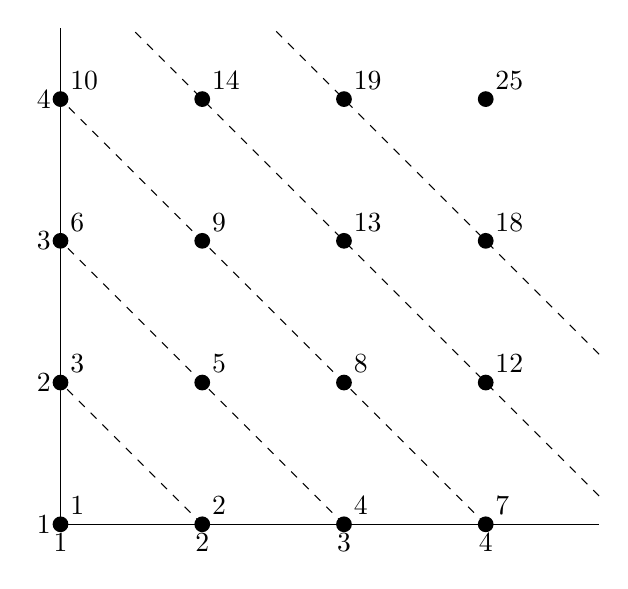
\begin{tikzpicture}[scale=1.8]
      \draw (0, 0) -- (0, 3.5);
      \draw (0, 0) -- (3.8, 0);
      \foreach \i in {1, 2, 3, 4} {
        \node [left] at (0, \i - 1) {\i};
        \node [below] at (\i - 1, 0) {\i};
      }

      \foreach \i in {1, 2, 3, 4} {
        \foreach \j in {1, 2, 3, 4} {
          \node [circle, fill = black, minimum size = 0.2cm, inner sep = 0] at (\i - 1, \j - 1) {};
          \node [anchor = south west] at (\i - 1, \j - 1) {\pgfmathparse{(\i + \j)*(\i + \j - 1) / 2 - \i + 1}\pgfmathprintnumber{\pgfmathresult}};
        }
      }

      \draw [dashed] (1, 0) -- (0, 1);
      \draw [dashed] (2, 0) -- (0, 2);
      \draw [dashed] (3, 0) -- (0, 3);
      \draw [dashed] (3.8, 0.2) -- (.5, 3.5);
      \draw [dashed] (3.8, 1.2) -- (1.5, 3.5);
    \end{tikzpicture}
  \end{center}
\end{proof}

Since $\Z$ is countable, we have an injection $\Z\to \N$, so there is an injection from $\Z\times \N\to \N\times \N \to \N$. So $\Z \times \N$ is countable. However, the rationals are the equivalence classes of $\Z\times\N$. So $\Q$ is countable.

\begin{prop}
  If $A\to B$ is injective and $B$ is countable, then $A$ is countable (since we can inject $B \to \N$).
\end{prop}

\begin{prop}
  $\Z^k$ is countable for all $k\in \N$
\end{prop}

\begin{proof}
  By induction: $\Z$ is countable. If $\Z^k$ is countable, $\Z^{k + 1} = \Z\times \Z^k$. Since we can map $\Z^k \to \N$ injectively by the induction hypothesis, we can map injectively $\Z^{k + 1}\to \Z\times \N$, and we can map that to $\N$ injectively. 
\end{proof}

\begin{thm}
  A countable union of countable sets is countable.
\end{thm}

\begin{proof}
  Let $I$ be a countable index set, and for each $\alpha \in I$, let $A_\alpha$ be a countable set. We need to show that $\bigcup_{\alpha\in I} A_\alpha$ is countable. It is enough to construct an injection $h: \bigcup_{\alpha\in I} A_\alpha \to \N\times \N$ because $\N\times\N$ is countable. We know that $I$ is countable. So there exists an injection $f: I\to \N$. For each $\alpha\in I$, there exists an injection $g_\alpha: A_\alpha \to\N$.

  For $a\in \bigcup A_\alpha$, pick $m = \min\{j\in \N: a\in A_{\alpha}\text{ and }f(\alpha) = j\}$. This number exists by the well-ordering principle. Let $f(\alpha) = m$. ($\alpha$ is unique because $f$ is injective) Then $h(\alpha) = (m,g_\alpha(a))$ is an injection.
\end{proof}

\begin{prop}
  $\Q$ is countable.
\end{prop}
\begin{proof}
  It can be proved in two ways:
  \begin{enumerate}
    \item $\Q = \bigcup_{n\geq 1} \frac{1}{n}\Z = \bigcup_{n\geq 1} \left\{\frac{m}{n}: m\in \Z\right\}$, which is a countable union of countable sets.
    \item $\Q$ can be mapped injectively to $\Z\times \N$ by $a/b\mapsto (a, b)$, where $b > 0$ and $(a, b) = 1$.
  \end{enumerate}
\end{proof}

\begin{thm}
  The set of algebraic numbers is countable.
\end{thm}
\begin{proof}
  Let $\mathcal{P}_k$ be the set of polynomials of degree $k$ with integer coefficients. Then  $a_kx^k + a_{k - 1}x^{k - 1} + \cdots + a_0 \mapsto (a_k, a_{k - 1}, \cdots, a_0)$ is an injection $\mathcal{P}_k \to \Z^{k + 1}$. Since $\Z^{k + 1}$ is countable, so is $\mathcal{P}_k$.

  Let $\mathcal{P}$ be the set of all polynomials with integer coefficients. Then clearly $\mathcal{P} = \bigcup \mathcal{P}_k$. This is a countable union of countable sets. So $\mathcal{P}$ is countable.

  For each polynomial $p \in \mathcal{P}$, let $R_p$ be the set of its roots. Then $R_p$ is finite and thus countable. Hence $\bigcup_{p\in \mathcal{P}} R_p$, the set of all algebraic numbers, is countable.
\end{proof}

\begin{thm}
  The set of real numbers $\R$ is uncountable. 
\end{thm}

\begin{proof}
  (Cantor's diagonal argument) Assume $\R$ is countable. Then we can list the reals as $r_1,r_2,r_3\cdots$ so that every real number is in the list. Write each $r_n$ uniquely in decimal form (ie. without infinite trailing '9's). List them out vertically:
  \begin{align*}
    r_1 &= n_1\,.\,d_{11}\,d_{12}\,d_{13}\,d_{14}\cdots\\
    r_2 &= n_2\,.\,d_{21}\,d_{22}\,d_{23}\,d_{24}\cdots\\
    r_3 &= n_3\,.\,d_{31}\,d_{32}\,d_{33}\,d_{34}\cdots\\
    r_4 &= n_4\,.\,d_{41}\,d_{42}\,d_{43}\,d_{44}\cdots
  \end{align*}
  Define $r = 0\,.\,d_1\,d_2\,d_3\,d_4\cdots$ by $d_n = 
  \begin{cases}
    0 & d_{nn}\not= 0\\
    1 & d_{nn}=0
  \end{cases}$. Then by construction, this differs from the $n$th number in the list by the $n$th digit, and is so different from every number in the list. Then $r$ is a real number but not in the list. Contradiction.
\end{proof}

\begin{cor}
  There are uncountable many transcendental numbers.
\end{cor}

\begin{proof}
  If not, then the reals, being the union of the transcendentals and algebraic numbers, must be countable. But the reals is uncountable.
\end{proof}
\note This is an easy but non-constructive proof that transcendental numbers exists. ``If we can't find one, find lots!''

\begin{eg}
  Let $\mathcal{F}_k = \{Y\subseteq \N: |Y| = k\}.$ We can inject $\mathcal{F}_k \to \Z^k$ by $\{1, 3, 7\}\mapsto (1, 3, 7)$ etc. So $\mathcal{F} = \bigcup_{k\geq 0}\mathcal{F}_k$, the set of all finite subsets of $\N$ is countable.
\end{eg}

\begin{eg}
  Recall $\mathcal{P}(X) = \{Y: Y\subseteq X\}$. Now suppose $\mathcal{P}\N$ is countable. Let $S_1,S_2,S_3, \cdots$ be the list of all subsets of $\N$. Let $S = \{n: n\not\in S_n\}$. But then $S$ is not in the list. Contradiction. So $\mathcal{P}\N$ is uncountable.
\end{eg}

\begin{eg}
  Let $\Sigma$ be the set of all functions $\N\to \N$ (ie. the set of all integer sequences). If $\Sigma$ were countable, we could list it as $f_1, f_2, f_3\cdots$. But then $f$ given by $f(n) = 
  \begin{cases}
    1 & f_n(n) \not= 1\\
    2 & f_n(n) = 1
  \end{cases}$. Again $f$ is not in the list. So $\Sigma$ is uncountable.

  Alternatively, there is a bijection between $\mathcal{P}(\N)$ and the set of 0, 1 sequences by $S\mapsto$ the indicator function. So we can inject $\mathcal{P}\N \to \Sigma$ by $S\mapsto $ indicator function $+1$. So $\Sigma$ cannot be countable (since $\mathcal{P}\N$ is uncountable).

  Or, we can let $\Sigma^*\subseteq \Sigma$ be the set of bijections from $\N\to\N$. Let $\Sigma^{**}\subseteq \Sigma^*$ be the bijections of the special form: for every $n$,
  \[
    \text{either}
    \begin{cases}
      f(2n - 1) = 2n - 1\\
      f(2n) = 2n
    \end{cases}\text{, or }
    \begin{cases}
      f(2n - 1) = 2n\\
      f(2n) = 2n - 1
    \end{cases},
  \]
  ie. for every odd-even pair, we either flip them or keep them the same.

  But there is a bijection between $\Sigma^{**}$ and $0,1$ sequences: if the $n$th term in the sequence $ = 0$, don't flip the $n$th pair in the function, vice versa. Hence $\Sigma^{**}$ is uncountable. 
\end{eg}

\begin{thm}
  Let $A$ be a set. Then there is no surjection from $A\to \mathcal{P}A$. 
\end{thm}

\begin{proof}
  Suppose $f: A\to \mathcal{P}(A)$ surjectively. Let $S = \{a\in A: a\not\in f(a)\}$. Since $f$ is surjective, there must exist $s\in A$ such that $f(s) = S$. If $s\in S$, then $s\not\in S$ by the definition of $S$. Conversely, if $s\not\in S$, then $s\in S$. Contradiction. So $f$ cannot exist. 
\end{proof}

This shows that there are infinitely many different possible ``infinite sizes'' of sets.

\begin{thm}[Cantor-Schr\"oder-Bernstein theorem]
  Suppose there are injections $A\to B$ and $B\to A$. Then there's a bijection $A\leftrightarrow B$. 
\end{thm}

\noindent \textbf{Continuum hypothesis.} There is no set whose size lies between $\N$ and $\R$.
In 1963, Paul Cohen proved that it is impossible to prove this or disprove this statement (in ZFC).
\end{document}
